\chapter[Metodolog\'ia.]{Metodología}
\pagestyle{fancy}
%[ML] Aqu{i describiría un poco mas el PIV15, algo así como... y el caso de aplicación en el PIV15-177, proyecto denominado "Diseño y lalalala de tatatat", financiado por el Consejo Nacional de Ciencias y Tecnología (CONACYT}
En este cap\'itulo se describen las consideraciones tenidas en cuenta para el desarrollo de la sonda, el diseño mec\'anico, el\'ectrico, electr\'onico, control y comunicaci\'on de cada uno de los componentes que componen la sonda y su sistema de despliegue. Adem\'as de los diagramas, algoritmos de funcionamiento y el caso de aplicaci\'on en el PINV15-177.

\section[Consideraciones del sistema]{Consideraciones de Dise\~no}
Para el desarrollo de la soluci\'on propuesta, se tuvo en cuenta las siguientes consideraciones:
\begin{itemize}
   \item Portabilidad: Se espera que el tamaño y el peso de la sonda sean transportables con facilidad, el di\'ametro debe ser menor a 150 [mm].
    \item Asequibilidad: Se espera que el costo final pueda ser reducido en un 20\% del costo de una soluci\'on comercial parecida (Libelium Smart Water), valorada en aproximadamente \$ 3,800 (tres mil ochocientos d\'olares americanos), sin contar los impuestos y gastos de importaci\'on, \cite{storeLibelium}.  
    \item Escalabilidad: Se espera que la solución pueda ser escalable y configurable según la necesidad, permitiendo la incorporación de otros tipos de sensores. Vers\'atil para que pueda ser compatible con otros sensores con peque\~nos o ningún cambio en la sonda.
    \item Compatibilidad: Se espera que la sonda pueda ser compatible con varios protocolos de comunicaci\'on y con otros sensores, con la menor cantidad de adaptaciones mec\'anicas o electr\'onicas. 
    \item Rangos de medici\'on: Considerando que el lugar de despliegue de la sonda, ser\'a en el lago Ypacaraí, se espera que la soluci\'on pueda desenvolverse sin problemas hasta 4 metros de profundidad, considerando el estudio de batimetr\'ia realizado por el laboratorio de Soluciones tecnol\'ogicas para la gesti\'on Integral de los Recursos H\'idricos,\cite{itaipu-binacional-2014}.
    \item Adaptabilidad: Se espera que la soluci\'on pueda ser utilizada con diferentes sistemas de despliegue.
    \item \textit{Open Source}: Se espera que durante el desarrollo de la soluci\'on se prioricen los sistemas open source para reducir costos y poder contribuir al ecosistema. 
    \item Autonom\'ia: Se espera que la soluci\'on presentada se pueda utilizar sin necesidad de estar sujeto a otros sistemas, y equipado con una fuente de alimentaci\'on independiente y recargable que permita el muestreo de al menos 10 horas de forma continua, que es la duraci\'on promedio de luz natural, \cite{ClimaSol}. 
\end{itemize}
Teniendo en cuenta las consideraciones y criterios previamente expuestos, luego de la revisi\'on de los trabajos de otros autores, estudiados en las secciones anteriores. A continuaci\'on, se abordar\'a el proceso de desarrollo involucrado, esta secci\'on estará organizada de la siguiente forma, en primer lugar se realiza una descripci\'on de todo el sistema general, y luego se  describe cada uno de los elementos, todo el proceso dise\~no, en el cual se detallan los planos y diagramas m\'ecanicos de cada uno de los elementos del sistema en la subsecci\'on de dise\~nos m\'ecanicos, los diagramas, planos y esquemas de conexi\'on el\'ectrica en la subsecci\'on de dise\~no el\'ectrico, en la subsecci\'on de dise\~no electr\'onico se abarcará lo concerniente al diseño electr\'onico, circuitos de adquisici\'on de datos de los sensores, drivers y otros elementos, en la subsecci\'on de la base de datos y control.
\section{Descripci\'on  sistema }
En esta sección se describen cada uno de los sistemas que comprende el desarrollo de este TFG, como el m\'odulo de la sonda y el sistema del m\'odulo de despliegue.
En referencia al modelo conceptual del sistema, éste se encuentra constituido de forma modular, de manera a facilitar agregar nuevos m\'odulos seg\'un sean necesarios, como se puede apreciar en la figura \ref{fig:DiagramaGeneral}, en este trabajo se implementaron los subsistemas sonda, perif\'ericos y estación remota.  

\begin{figure}[H]
    \centering
    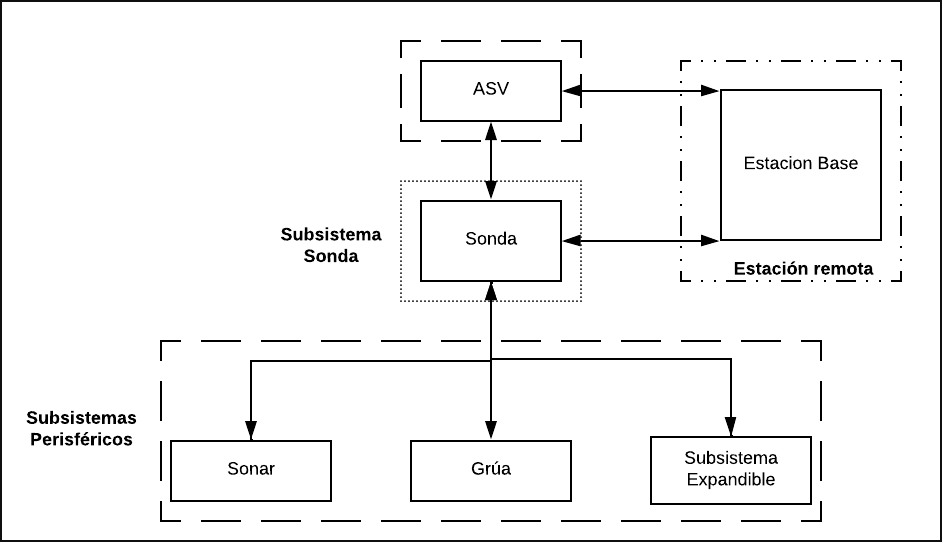
\includegraphics[scale=0.4]{Imagenes/cap1/Diagrama.png}
    \caption[Diagrama General del Sistema]{Diagrama General del Sistema. }{\textbf{Fuente:} Elaboración Propia.}
    \label{fig:DiagramaGeneral}
\end{figure}

A continuación se describen los subsistemas.
\begin{itemize}
    \item \textbf{Subsistema Sonda}: subsistema principal y punto central de comunicaci\'on de los dem\'as subsistemas, este permite el control de los diferentes sensores para monitorio, as\'i como el almacenamiento en base de datos y transmisión de los resultados del muestreo obtenido.
    \item \textbf{Subsistema Perif\'ericos}: subsistemas secundarios, encargados de agregar las capacidades necesarias para lograr los objetivos de muestreo, para el muestreo a multinivel se desarrollaron los subsistemas Radar, para medir la profundidad; Gr\'ua, para lograr desplazamiento vertical de descenso y ascenso la sonda; ASV, para el desplazamiento horizontal de la sonda y las coordenadas GPS de los puntos de  muestreo. 
    \item \textbf{Estaci\'on remota}: destino principal de retransmisi\'on de los datos recolectados de la sonda. 
\end{itemize}

\subsection[Descripción General del Sistema]{Descripción General del Sistema}
En la figura \ref{fig:diagramaSecuencia} se puede apreciar la secuencia de operaci\'on de cada uno de los elementos que componen el trabajo desarrollado; la sonda fue dise\~nada para ser incorporada en el asv del proyecto PIN15-177, la secuencia de operaci\'on inicia desde el ASV cuando llega al punto de muestreo. 
Una vez que el ASV da la orden de inicio, la sonda recibe la petici\'on y solicita al sonar la profundidad en ese punto, el valor de la profundidad de ese punto en cent\'imetros retorna a la sonda, la sonda realiza un c\'alculo donde se limita la profundidad m\'axima de descenso y el valor resultante es enviado a la gr\'ua e inicia el proceso de muestreo que consiste en solicitar a los sensores de forma secuencia sus lecturas en intervalos de 5 segundos, la secuencia de lectura de los sensores se almacena directamente en una base de datos local del raspberry, los datos recolectados se trasmite v\'ia protocolo de comunicaci\'on MQTT. 
Con el dato recibido en la grúa se ejecuta al algoritmo de descenso teniendo en cuenta el valor de profundidad, el algoritmo genera al menos dos profundidades(menores a 30 cm) de parada, donde la gr\'ua se detiene por un intervalo de 30 segundos, una vez que la gr\'ua desciende hasta la profundidad calculada, el mismo realiza la operaci\'on de ascenso, cuando culmine al algoritmo manda un estatus verdadero al la sonda que lo interpreta como secuencia finalizada.
La sonda, al recibir la confirmaci\'on  de la gr\'ua, configura todos los sensores a modo sleep, y envía una se\~nal al ASV para indicar que finalizó el muestreo en ese punto, para que el ASV pase a uno siguiente donde se repite la secuencia. 

\begin{figure}[H]
    \centering
    \includegraphics[width=\textwidth]{Imagenes/cap3/Diagrama de secuencia básico.png}
    \caption {Diagrama de secuencia de operaci\'on.}{\textbf{Fuente:}
    Elaboraci\'on Propia. }
    \label{fig:diagramaSecuencia}
\end{figure}

\subsection[Caracter\'isticas T\'ecnicas del m\'odulo despliegue]{Caracter\'isticas T\'ecnicas del m\'odulo despliegue}
La Tabla \ref{tab:carac_general} detalla las caracter\'isticas t\'ecnicas del mecanismo a ser desarrollado, teniendo en cuenta los objetivos planteados en la  \autoref{Objetivos}.

\begin{table}[H]
\protect\caption[Datos T\'ecnicos m\'odulo despliegue]{Datos T\'ecnicos m\'odulo despliegue. \label{tab:carac_general}}
    \centering
    \scalebox{0.9}{\begin{tabular}{c c}
        \textbf{Caracter\'istica} & \textbf{Valor}  \\
        \hline
        \multicolumn{2}{l}{\textbf{F\'isico}} \\
        Capacidad de carga & $ > 10 [Kg] $   \\
        Dimensiones & $< 50 [cm]$  x $50 [cm]$ x $50 [cm]$    \\
        Peso &  $ < 15 kg$ \\
        Caja Electr\'onica & Herm\'etica  \\
        \multicolumn{2}{l}{\textbf{Eléctrico}} \\
         Alimentaci\'on & 12 V DC  \\
         Autonom\'ia & No  \\
         \multicolumn{2}{l}{\textbf{Interfaz}} \\
         Configuraci\'on de Par\'ametros & Por Interfaz Gr\'afica  \\
         Transmisi\'on Remota  & Si  \\
        \hline
    \end{tabular}}
    \vspace{5mm}
    \newline
    \hfill \textbf{Fuente:} Elaboraci\'on Propia
\end{table}
Por motivos energ\'eticos, el m\'odulo de despliegue no debe ser muy pesado, para no sobrecargar m\'as su funcionamiento, ya que el ASV posee elementos muy pesados, pero imprescindibles para el funcionamiento.
Por el diseño el\'ectrico adoptado y las configuraciones de los drivers de carga, la alimentación debe de ser de 12 VDC, donde la autonom\'ia esperada es la misma que el ASV. Todos los sistemas que integran este m\'odulo deben de comunicarse entre s\'i para efectuar procesos automatizados combinados, pero tambi\'en debe ser posible alg\'un tipo de intervenci\'on manual en caso de emergencia, por situaciones no previstas y donde se requiera un tipo de interacci\'on humano - máquina, para ello también debe de ser posible su control mediante el uso de una interfaz que sea simple e intuitivo.

\subsection[Características Técnicas del m\'odulo Sonda]{Características Técnicas del m\'odulo Sonda}
La Tabla \ref{tab:carac_general2} detalla las características técnicas del mecanismo a ser desarrollado, teniendo en cuenta los objetivos planteados en la \autoref{Objetivos}
\begin{table}[ht]
% \protect
    \caption[Datos Técnicos m\'odulo sonda]{Datos Técnicos m\'odulo sonda.}
    \label{tab:carac_general2} 
    \centering
    % \scalebox{0.9}
    {\begin{tabular}{c c}
        % \hline
        \textbf{Característica} & \textbf{Valor}  \\
        \hline
        \multicolumn{2}{l}{\textbf{Sensores}} \\
        % \hline
        Cantidad & $ 5 $   \\
        % \hline
        \multicolumn{2}{l}{\textbf{Físico}} \\
        % \hline
        Dimensiones & $< 50 [cm]$  $< \phi 15[cm]$   \\
        % \hline
        Peso &  $ > 6 kg$ \\
        % \hline
        Caja Electrónica & Herm\'etica  \\
        % \hline
        \multicolumn{2}{l}{\textbf{Eléctrico}} \\
        % \hline
         Alimentación & 5 V DC  \\
        % \hline
         Autonomía & LiPo 5100mAh  \\
        % \hline
         \multicolumn{2}{l}{\textbf{Interfaz}} \\
        %  \hline
         Configuración de Parámetros & Por Interfaz Gráfica, SSH, VNC  \\
        % \hline
         Transmisi\'on Remota  & Si  \\
        \hline
    \end{tabular}}
    \vspace{5mm}
    \newline
    \hfill \textbf{Fuente:} Elaboración Propia
\end{table}

\subsection{Comunicaci\'on}
En la propuesta diseñada, se sugiere el desarrollo de varios subsistemas auxiliares para poder escalar y agregar nuevas capacidades o caracter\'isticas, seg\'un sea necesario.
Con la existencia de estos subsistemas que realicen procesos automatizados, se debe prever un sistema de comunicaci\'on que funcione correctamente bajo un esquema M2M (\textit{machine to machine}) e implementable bajo la tecnolog\'ia IoT (\textit{Internet Of The Things}). 
Bajo estas consignas, una de las tecnolog\'ias m\'as acordes fue \textit{Message Queing Telemetry Transport} (MQTT), que es un est\'andar OASIS para conectividad IoT, un protocolo de mensajer\'ia de publicaci\'on/suscripci\'on extremadamente simple y liviano, dise\~nado para dispositivos restringidos y redes de bajo ancho de banda. Los principios de dise\~no son minimizar el ancho de banda de la red y los requisitos de recursos del dispositivo, al mismo tiempo que intentan garantizar la confiabilidad y cierto grado de garant\'ia de entrega, \cite{mqtt-no-date}. Estos principios tambi\'en hacen que el protocolo sea ideal para el mundo de los dispositivos conectados del ``Internet de las cosas", y para las aplicaciones m\'oviles donde el ancho de banda y la energ\'ia de bater\'ia es limitada.
Los elementos b\'asicos de este protocolo y su interacci\'on est\'an representados en la figura  \ref{fig:mqtt}, a continuaci\'on una descripci\'on de cada uno de ellos:
  \begin{figure}[ht]
        \centering
        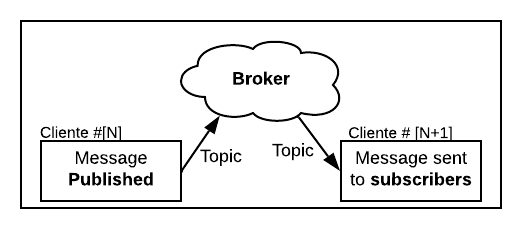
\includegraphics[scale=0.6]{Imagenes/cap3/Esquema Mqtt.png}
        \caption[Esquema b\'asico mqtt]{Esquema b\'asico mqtt}\textbf{Fuente:} Elaboraci\'on Propia.
        \label{fig:mqtt}
    \end{figure}
    
\begin{itemize}
    \item \textbf{Broker} – El \textit{broker} es el servidor que distribuye la información a los clientes interesados conectados al servidor.
    \item \textbf{Client} – Cliente, es el dispositivo que se conecta al \textit{broker} para enviar o recibir información.
    \item \textbf{Topic}- T\'opico, es el nombre de la ruta que etiquetan los dispositivos. Los clientes publican, se suscriben o hacen ambas cosas a un tema.
    \item \textbf{Publisher} – El publicador es el que envía los datos del cliente  al \textit{broker} para distribuir a los clientes interesados bas\'andonos en el nombre del t\'opico.
    \item \textbf{Subscribers} – El suscriptor es el nombre que reciben los  clientes, con el cual reciben los mensajes asociados según el t\'opico. Cuando un cliente se suscribe a un t\'opico, cualquier mensaje publicado al \textit{broker} es distribuido a los suscriptores de ese t\'opico. Los clientes también pueden cancelar la suscripción para dejar de recibir mensajes del \textit{broker} sobre ese tópico.
\end{itemize}

Considerando los elementos anteriormente expuestos, el sistema de comunicaci\'on 
se implement\'o en dos niveles, una a nivel local y otra a nivel remoto, mediante servidores distintos con t\'opicos de mensajes independientes. 
Un servidor local para tener un sistema robusto de intercambio de mensajes entre los subsistemas que no requiere de una conexi\'on estable a Internet; y un servidor remoto que depende de una conexi\'on a Internet para la transmisi\'on de datos recolectados a una estación remota ubicada en cualquier parte del mundo. 
Para ello fue necesario la elaboraci\'on de un diccionario de t\'opicos para establecer las rutas de informaci\'on y de esta forma lograr la conexi\'on de cada uno de los sistemas.
El servicio de \textit{broker} utilizado como \textit{broker} remoto y como \textit{broker} local, es el servidor mosquitto desarrollado por la fundaci\'on Eclipse \cite{mosquitto_eclipse_2018}, Mosquitto es un intermediario de mensajes de código abierto (con licencia EPL/EDL) que implementa las versiones 5.0, 3.1.1 y 3.1 del protocolo MQTT. Mosquitto es liviano y adecuado para su uso en todos los dispositivos, desde computadoras de placa única como el Raspberry Pi de bajo consumo hasta servidores dedicados.
\begin{figure}[ht]
        \centering
        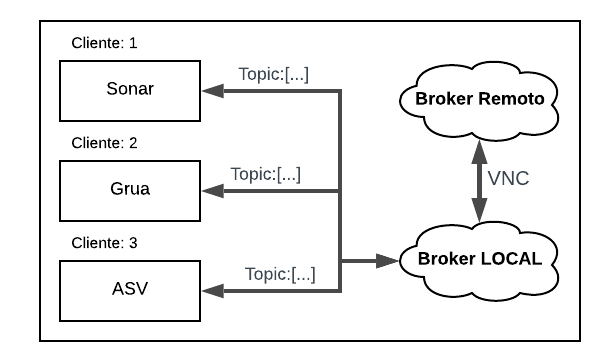
\includegraphics[scale=0.6]{Imagenes/cap3/esquemaCom.png}
        \caption[ Esquema configuraci\'on mqtt]{Esquema configuraci\'on}\textbf{Fuente:} Elaboración Propia.
        \label{fig:mqttUtil}
    \end{figure}

El esquema de comunicaci\'on, implementado en este trabajo, ver en la figura \ref{fig:mqttUtil}, est\'a compuesto por 3 (tres) clientes conectados al servidor local y un servidor remoto. La cantidad de clientes responde directamente a la cantidad necesaria de perif\'ericos a ser instalados, pudiendo ampliarse para otorgarle alg\'un nuevo tipo de funcionalidad. 

\begin{itemize}
    \item \textbf{Cliente 1: Sonar} – Este cliente corresponde al subsistema auxiliar encargado de medir la profundidad en el punto de muestreo,  esta informaci\'on ser\'a utilizado para el registro en base de datos y publicando para los dem\'as clientes mqtt.
    \item \textbf{Cliente 2: Gr\'ua} – Este cliente corresponde al siguiente subsistema encargado del desplazamiento vertical de la sonda, con el dato publicado del cliente 1, calcula los desplazamientos a ser realizados.
    \item \textbf{Cliente 3:ASV}- Este cliente corresponde al subsistema que otorga el desplazamiento horizontal a la sonda, publica los datos de telemetr\'ia correspondientes al ASV y publica la ubicaci\'on GPS registrado en el momento de la extracci\'on de la muestra.
\end{itemize}

Para la conexi\'on entre el servidor remoto y el servidor local ser utiliza OpenVPN, que es un software open source basado en VPN. La VPN (Virtual Private Network) significa red privada virtual. Es un t\'unel encriptado entre dos dispositivos que permite acceder a cada sitio web y servicios en línea de forma privada y segura, es capaz de conectar uno o más dispositivos como si se encontraran físicamente en la misma red local (LAN) y en el mismo lugar, \cite{arora_131_nodate}. Al momento de conectarse a una VPN, se crea un “túnel” entre los diapositivos mediante la conexi\'on a internet, los datos siempre permanecerán cifrados, y accesibles \'unicamente mediante certificados de conexi\'on generados en el programa. 

\section{Sonda}
El dise\~no final fue un proceso evolutivo resultado de varias iteraciones iniciado en el proyecto Cormor\'an-I detallado en \'el 
\nameref{appendix: cormoran}
, partiendo del modelo utilizado por Hitz y otros,\cite{hitz2012design}
hasta la versi\'on final, aunque esta soluci\'on est\'a pensada principalmente para el proyecto PIN15-177, la idea de este trabajo es contar con un dispositivo capaz de funcionar de forma independiente a cualquier otro tipo de veh\'iculo, extendiendo as\'i sus posibles tipos de usos, como el monitoreo de acu\'iferos, ésto supone que la sonda deba contar con todos los elementos necesarios para su correcto desenvolvimiento, la funci\'on principal de la sonda es brindar soporte a cada uno de los sensores, el soporte incluye el procesamiento de se\~nal, alimentaci\'on, almacenamiento de datos, protecci\'on contra impactos y transmisi\'on a una estaci\'on base remota los datos sensados.
\begin{table}[ht]
\protect\caption[Funciones Generales]{Funciones Generales. \label{tab:fun_general}}
    \centering
    \begin{tabular}{l l l}
        \toprule
        \textbf{Descripción} & \textbf{Decisión} & \textbf{Característica} \\
        \midrule
         Comunicaci\'on  Perif\'ericos  & Algoritmo comunicaci\'on & \multicolumn{1}{ l}{\begin{tabular}[c]{@{}l@{}} Env\'io y recipci\'on de estados \\ funcionamiento y datos de los \\ dispositivos conectados a la red \end{tabular}}
         \\ \\
%        \hline
        Lectura de Sensores & Algoritmo muestreo & \multicolumn{1}{l}{\begin{tabular}[c]{@{}l@{}} Se Lectura secuencial de los\\ sensores pH, CE,\\ OD, OPR, T\end{tabular}}
         \\ \\
%        \hline
        Almacenamiento datos & Algoritmo datos &
        \multicolumn{1}{l}{\begin{tabular}[c]{@{}l@{}} Consulta y registro as\'incrono \\ 
        del muestreo\end{tabular}}
         \\ \\
%        \hline
        Transmisi\'on datos  & Algoritmo transmisi\'on &
        \multicolumn{1}{l}{\begin{tabular}[c]{@{}l@{}} Transmisi\'on asincr\'onica \\ a estaci\'on remota \end{tabular}}
           \\
        \bottomrule
    \end{tabular}
    \vspace{5mm}
    \newline
    \hfill \textbf{Fuente:} Elaboración Propia
\end{table}
Para el proyecto PIN15-177, la sonda a ser implementada debe dar soportes inicialmente a cinco sensores (ph, CE, OD, OPR, T), y el dise\~no debe soportar la incorporaci\'on y/o retiro de alg\'un sensor, sin que esto conlleve adaptaciones importantes en la sonda, por ese motivo se opt\'o por un dise\~no modular de tal forma que, cuando sea necesario modificar alg\'un sensor se tenga que reemplazar simplemente uno de los m\'odulos y de esta forma reducir los costos. Los tres mo\'dulos est\'an compuestos por:
\begin{itemize}
    \item \textbf{Frente}: Este m\'odulo es la pieza frontal de la sonda, cuya funci\'on principal es de protecci\'on a cada uno de los sensores contra basuras u objetos con que puede entrar en contacto directo y ,adem\'as, crear un entorno de volumen de agua constante y reducir en la mayor medida posible la formaci\'on de turbulencias alrededor de los sensores para evitar los fallos o errores de lecturas de los sensores que se podr\'ian registrar a causa de burbujas de aire en los cabezales de los sensores. Tal como indica en la figura \ref{fig:Frente}, la zona comprendida dentro del recuadro rojo. As\'i como se indica en el plano del anexo \ref{fig:ModuloFrontal}, para el dise\~no de est\'e m\'odulo, se parti\'o de una forma cil\'indrica hueco de altura suficiente para poder cubrir totalmente cada uno de los sensores, con aberturas longitudinales equidistantes en las paredes laterales en forma de ranuras con bordes redondeados, una de las bases totalmente libre para que se pueda acoplar a los otros m\'odulos, y  la otra base redondeada de forma esf\'erica y hueca, a fin favorecer el efecto hidrodin\'amico al momento del contacto con el agua, como se presentara m\'as adelante con las simulaciones realizadas.
    
    \begin{figure}[ht]
        \centering
        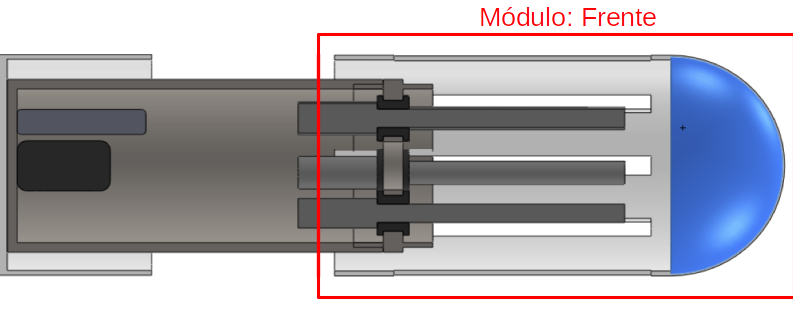
\includegraphics[width=110mm, height=40mm]{Imagenes/cap3/CompletoV5_Frente.png}
        \caption[Corte Transversal]{Corte Transversal Sonda. M\'odulo: Frente.}\textbf{Fuente:} Elaboración Propia.
        \label{fig:Frente}
    \end{figure}
    \item \textbf{Base}: Este m\'odulo, es la parte posterior de la sonda, su función principal es almacenar de forma segura todo el equipamiento electr\'onico de control, el\'ectrico, alimentación y placas necesarias para los sensores, tal como se indica en la figura \ref{fig:Base2020}, la base est\'a conformada por un cilindro hueco de 270 [mm] de altura, 120[mm] de di\'ametro exterior, espesor de las paredes internas laterales de 10[mm] y un espesor de la base 15[mm],  para sellar de forma herm\'etica, se utilizó un roscado Whitworth fino, utilizada para tuber\'ias de gas y de agua, \cite{falk_metalotecnia_1986}, de paso 1,154 [mm].
    
    \begin{figure}[H]
    \centering
    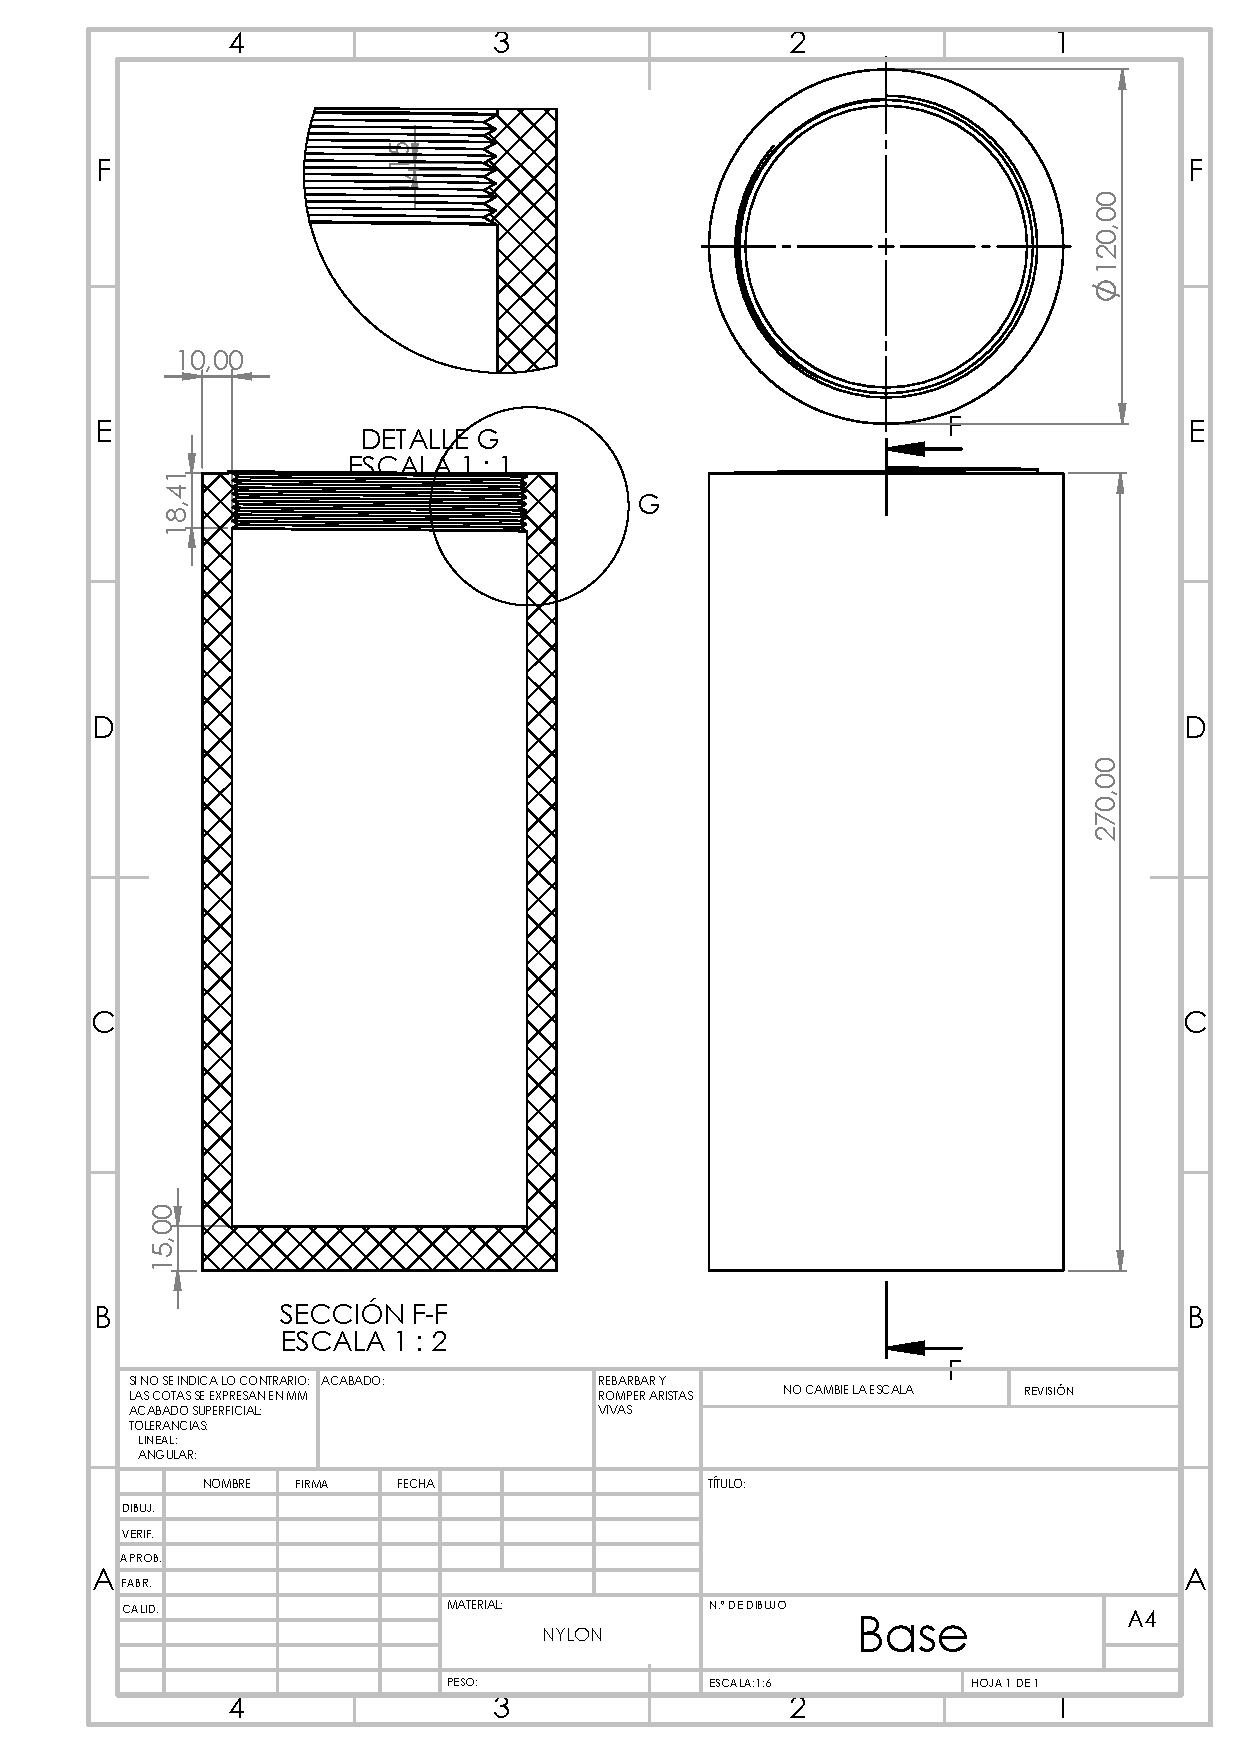
\includegraphics[width=\linewidth]{Imagenes/2019/Base2019.PDF} 
    \caption{Dise\~no final de la base.}{ \textbf{Fuente}: Elaboraci\'on propia}
    \label{fig:Base2020}
    \end{figure}
    
    \item \textbf{Anillo}: Tercer
    m\'odulo, es la parte central de la sonda, adem\'as de servir como enlace 
    entre las otras dos piezas, tiene dos funciones principales; en primer lugar acoplarse a la base cerr\'andolo de forma herm\'etica y la segunda de sostener los sensores en sus posiciones fijas en la sonda. Este es el m\'odulo m\'as peque\~no en relaci\'on a los otros dos, se diseñó de esta forma para ser el \'unico m\'odulo que se espera que se tenga que reemplazar en el caso de ser necesario una reconfiguraci\'on u modificaci\'on de los sensores. Tal como se muestra en la figura \ref{fig:Anillo2019} el dise\~no parte de un cilindro macizo de 70 [mm] de altura y 120[mm] de di\'ametro exterior, se utiliz\'o Whitworth fino al igual que la base a fin de que pueda enroscarse  perfectamente, con el roscado se asegura hasta cierto punto el cierre herm\'etico entre los dos m\'odulos, como medida de seguridad extra se introducen los o-ring, para crear otro  sello hermético al momento del contacto entre las dos m\'odulos, con estos dos sistemas se espera que el ingreso de l\'iquidos sea nulo o m\'inimo, para la implementaci\'on de la sonda en este trabajo se utilizan 5 sensores, y como esta secci\'on es la encargada de mantener en su posici\'on cada uno de los sensores, se realizan cinco perforaciones en este m\'odulo a fin de poder colocarlos de forma perpendicular. Como estas perforaciones para los sensores implicar\'ia posibles \'areas de ingreso de l\'iquido, considerando adem\'as que el uso de o-ring se tornan un poco complicados para la posterior fabricaci\'on, se opt\'o por utilizar juntas hidr\'aulicas estandarizadas con el di\'ametro interno compatible con el di\'ametro del los sensores, dispuesta en pares por cada uno de los sensores a fin de sellar las perforaciones y con esto impedir el ingreso de líquidos al interior de la sonda.
    
    \begin{figure}[H]
        \centering
        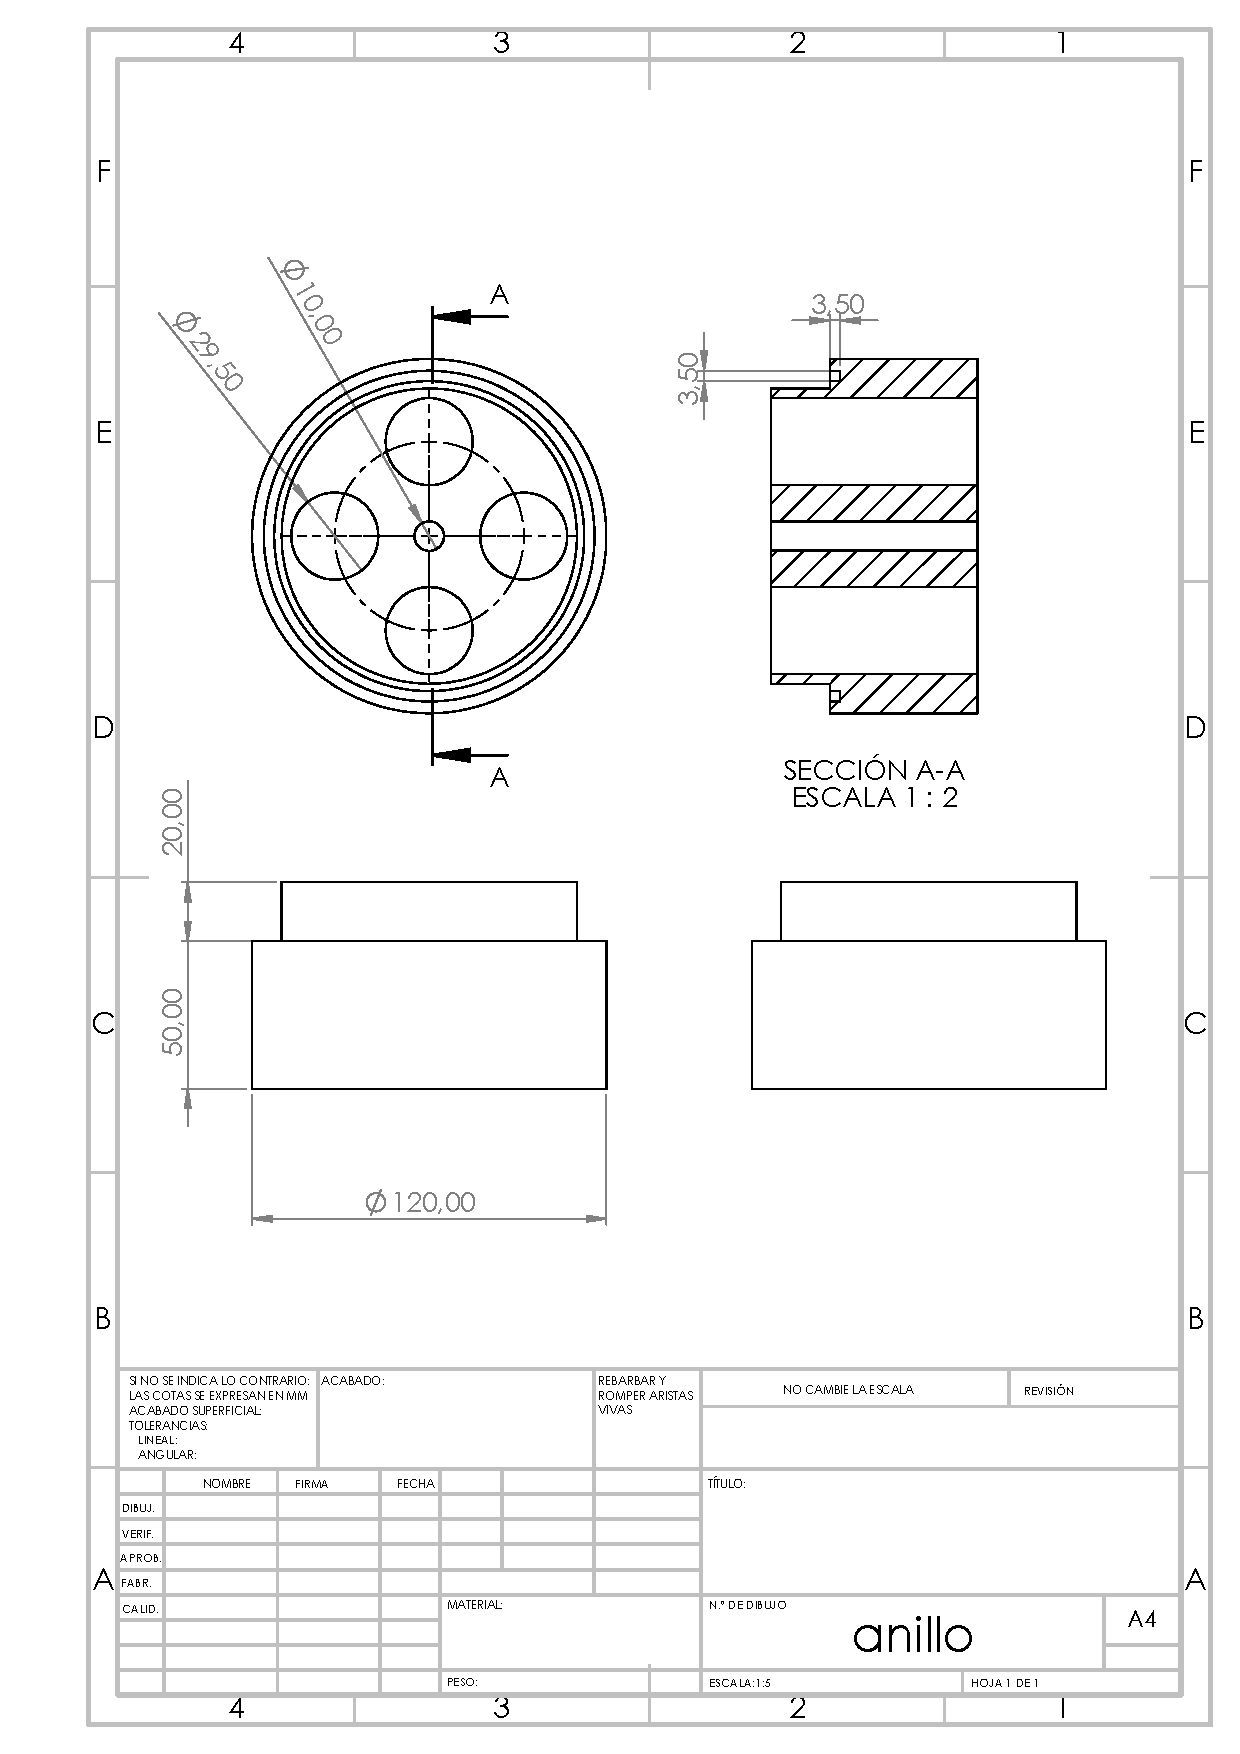
\includegraphics[width=\linewidth]{Imagenes/2019/anillo2019.PDF} 
        \caption{Dise\~no final del anillo. Fuente: elaboración propia}
        \label{fig:Anillo2019}
        \end{figure}
    \end{itemize}

% parte Electrica 
Para lograr autonom\'ia energ\'etica para la sonda se opt\'o por utilizar bater\'ias LiPo Nano-Tech por sus caracter\'isticas t\'ecnicas que permitir\'an alimentar de forma suficiente a toda los componentes que conforman la sonda, como se aprecia en la figura \ref{fig:nanoBateria}, es posible conectar dos baterías en serie para lograr obtener el nivel energético 2S, para que pueda funcionar el sistema.  
    \begin{figure}[H]
        \centering
        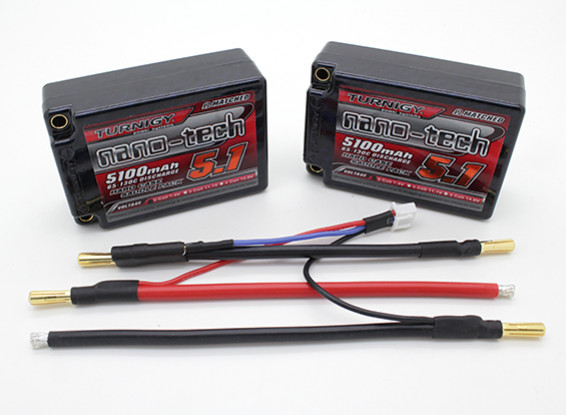
\includegraphics[width=0.4\textwidth]{Imagenes/2021/imag29.jpg}
        \caption{Baterias NanoTech Turnigy 5100 mAh}\textbf{Fuente:} P\'agina web del fabricante,\cite{bateria}.
        \label{fig:nanoBateria}
    \end{figure}
Las bater\'ias Turnigy nano-tech Lipoly bater\'ias fueron dise\~nadas para alto rendimiento, utilizando un avanzado sustrato electrones que permite pasar m\'as libremente de \'anodo a c\'atodo con menos impedancia interna.
 
Las ventajas sobre las bater\'ias tradicionales LIPOLY:
\begin{itemize}
    \item La densidad de potencia alcanza 7,5 kW / kg.
    \item Menos hueco de tensi\'on durante la descarga de alta velocidad, dando m\'as poder bajo carga.
    \item Impedancia interna puede llegar tan bajo como 1.2 m${\Omega }$ en comparación con la de 3 m${\Omega }$ de un Lipoly estándar.
    \item Hinchazón durante la carga pesada no supera 5\%, en comparación con 15\% de un Lipoly normal.
    \item Mayor capacidad durante la descarga pesada. M\'as del 90\% a la tasa de 100 \% C.
    \item Carga r\'apida hasta 15$^{\circ}$C en algunas baterías.
    \item Mayor duraci\'on del ciclo, casi el doble que el de la tecnolog\'ia LiPoly est\'andar.
\end{itemize}

La tecnolog\'ia de nano-core en las bater\'ias de litio es la aplicaci\'on de aditivos conductores nan\'ometros. Los aditivos nan\'ometros conductora forman redes ultra-fuertes de electrones de conducci\'on en los electrodos que pueden aumentar la conductividad electr\'onica.
Estos aditivos crean la capacidad de imbibici\'on en el l\'iquido portador para suministrar m\'as canales de iones. Esto mejora la capacidad de transmisi\'on de iones y la difusi\'on de iones. A trav\'es de la mejora de la conductividad y de iones de transmisi\'on electr\'onica, la impedancia se reduce y la polarizaci\'on de la descarga de alta tasa disminuye en gran medida.
\begin{table}[t]
\protect\caption[Caracter\'isticas de bater\'ia Lipo Nano-Tech ]{Caracter\'isticas de bater\'ia Lipo Nano-Tec 5100 mAh.}
\label{tab:caract_bat}
\begin{center}
\begin{tabular}{l l}
\hline
Capacidad    &  5100 mAh \\
Voltaje      &  2S3P/ 7.4 V \\
Descarga &  65C / 135C \\
Peso  & 290 g\\
Dimensi\'on   &  69x47x25 mm\\
Conector equilibrio	& JST\\
\hline
\end{tabular}
\vspace{5mm}
\newline
\hfill \textbf{Fuente:} P\'agina Web del Fabricante\cite{bateria}
\end{center}
\end{table}
\paragraph {Interfaz de Sensores}:
Es el bloque donde se obtiene las mediciones de las caracter\'isticas f\'isico - qu\'imicas del recurso h\'idrico para su posterior procesamiento, almacenamiento y transmici\'on a base remoto.
\subparagraph{Sensor de pH}
En la Figura \ref{fig:sensorpH}: se puede apreciar el sensor de pH por el que se optó fabricado por la empresa Atlas Scientfic.
Los criterios para la selección de este sensor fueron su simplicidad de uso debido a su extensa documentación y soporte por parte del fabricante, su popularidad en el ámbito de la automatización y control de calidad de agua para varios tipos de usos y su integración dentro de la placa de desarrollo sin necesidad de cableados externos y compatible con el módulo EZO pH Circuit que se muestra en la Figura \ref{fig:EZOpH}

\begin{figure}[H]
\caption[Sensor y EZO de pH.]{Sensor y EZO de pH de la empresa Atlas Scientific. }
     \centering
     \begin{subfigure}[b]{0.6\textwidth}
         \centering
         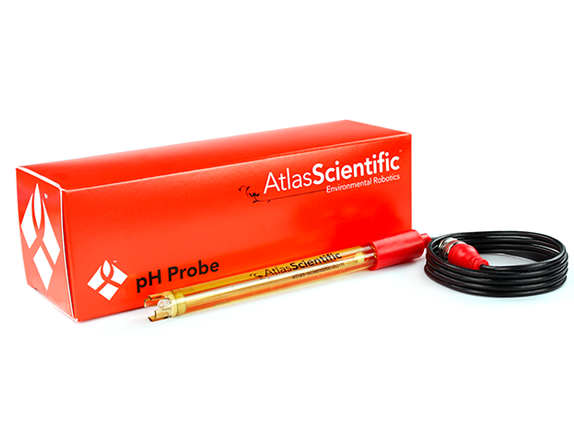
\includegraphics[width=\textwidth]{Imagenes/2021/imag23.png}
	    \caption[Sensor de pH.]{Sensor de pH. }
        \label{fig:sensorpH}
     \end{subfigure}
     \hfill
     \begin{subfigure}[b]{0.35\textwidth}
         \centering
         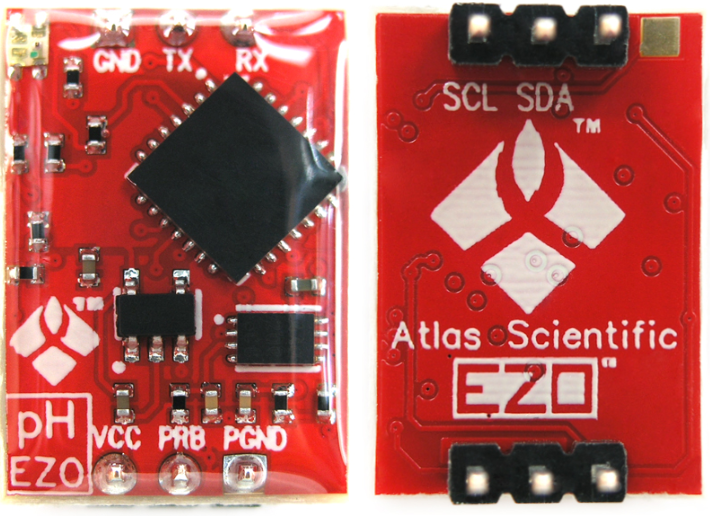
\includegraphics[width=\textwidth]{Imagenes/2021/imag27.png}
         \caption[EZO pH Circuit]{EZO pH Circuit.}
        \label{fig:EZOpH}
     \end{subfigure}
     {\textbf{Fuente:} P\'agina Web del Fabricante\cite{atlasph}.}
     \hfill
\end{figure}

El m\'odulo es un dispositivo bastante sensible, y esta sensibilidad es lo que le da una excelente precisión. 
Significa que es capaz de leer micro voltajes que est\'an presentes en el agua de fuentes no naturales como bombas, v\'alvulas de solenoide u otras sondas o sensores, lo que ocasiona lecturas que fluctúan rápidamente o lecturas que están constantemente apagadas.
Al leer el pH y la conductividad u oxígeno disuelto juntos, el fabricante recomienda que los m\'odulos estén aislados eléctricamente de los demás circuitos, subsanados con la placa de Tentacle.
\newline
\hfill
\begin{figure}[H]
    \centering
    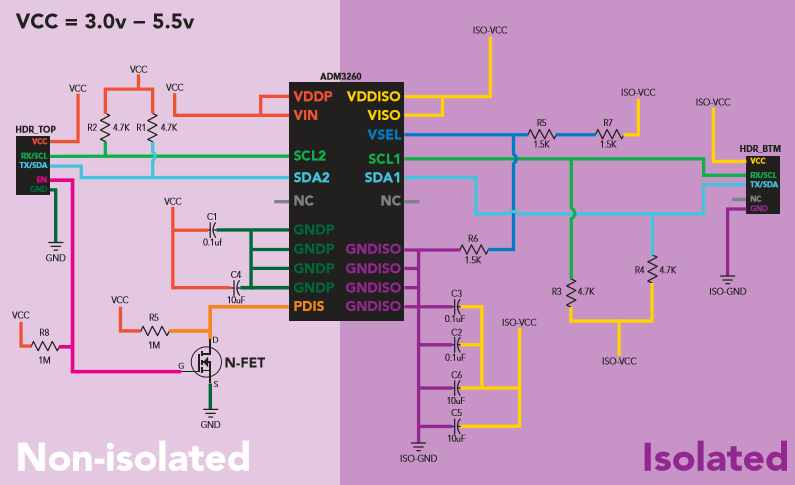
\includegraphics[width=\textwidth]{Imagenes/2021/imag36.png}
    \caption[Esquema de Funcionamiento del circuito EZO pH]{Esquema de Funcionamiento del circuito EZO pH.}{\textbf{Fuente:} P\'agina Web del Fabricante\cite{ezoph}.}
    \label{fig:4.10}
\end{figure}

En la Figura \ref{fig:4.10} se muestra  el esquema del circuito interno del módulo, cómo están aislados datos y la potencia con el ADM3260, que es el chip encargado de realizar la aislación de los canales I2C utilizados y algunos componentes pasivos. El ADM3260 puede generar una potencia aislada de hasta 150 mW e incorpora dos canales de datos bidireccionales.
Esta tecnología funciona mediante el uso de pequeños transformadores para inducir el voltaje a través de un espacio de aire. Los dos canales de datos tienen una resistencia de extracción de 4.7 $k\Omega$ tanto en las líneas aisladas como en las no aisladas (R1, R2, R3 y R4). El voltaje de salida se configura mediante un divisor de voltaje (R5, R6 y R, 7). produce un voltaje de 3.9 V independientemente de su voltaje de entrada.

\textbf{Principio de operación: }Una sonda de pH mide la actividad del ion de hidrógeno en un líquido, en el extremo inferior de ésta hay una membrana de vidrio que permite a los iones de hidrógeno del líquido que se está midiendo depositarse en la capa exterior del vidrio, mientras que los iones más grandes permanecen en la solución. En la Figura \ref{fig:phGrafico} se puede apreciar el comportamiento de los iones de hidrógeno de acuerdo al tipo de solución que se tiene. La diferencia en la concentración de iones de hidrógeno (fuera de la sonda y en el interior de la sonda) crea una corriente muy pequeña. Esta corriente es proporcional a la concentración de iones de hidrógeno en el líquido que se mide.
La corriente que se genera a partir de la actividad del ion hidrógeno es el recíproco de esa actividad y se puede predecir usando esta ecuación:
\begin{equation}
E=E^0 + \frac{RT}{F}\times \ln\alpha_{H+} = E^0 - \frac{2.303RT}{F}\rho H
\label{eq:iv}
\end{equation}
Donde $R$ es la constante ideal del gas, $T$ es la temperatura en grados Kelvin y $F$ es la constante de Faraday.
\newline
\hfill
\begin{figure}[H]
\centering
	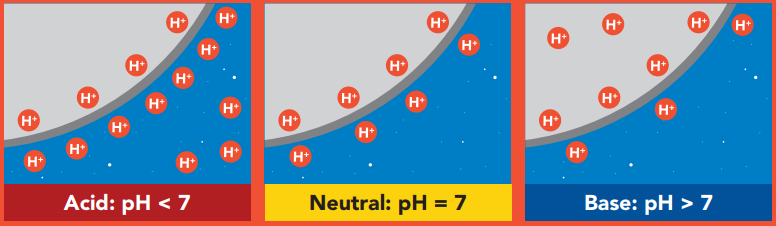
\includegraphics[width=\textwidth]{Imagenes/2021/imag22.png}%\textwidth%
	\caption[Actividad de los iones de hidrógeno]{Actividad de los iones de hidrógeno.  }{\textbf{Fuente:}P\'agina Web del Fabricante \cite{atlasph}}
	\label{fig:phGrafico}
\end{figure}

En la Tabla \ref{tab: caract_sondaph} se detallan las características del sensor de pH.
\newline
\hfill
Entre las aplicaciones típicas en las que se utiliza esta sonda están, uso estándar de laboratorio, uso en el campo, en el suelo, cultivos con técnicas de hidropon\'ia o acuapon\'ia, muestras que contienen metales pesados, cerveza, vino y otros.

\begin{table}[H]
\protect\caption[Características del sensor de pH de Atlas Scientific]{Características del sensor de pH de Atlas Scientific.}
\label{tab: caract_sondaph}
\begin{center}
\begin{tabular}{l l}
\hline
Rango    &  0 - 14\\
Exactitud      &  +/-0.002\\
Conector &  BNC macho\\
Resolución   &  +/-0.0001\\
Tiempo de Respuesta   &  95\% en 1 s\\
Presión Máxima    &  100PSI\\
Profundidad Máxima	& 60 m\\
Rango de Temperatura $^{\circ}$C	& 1- 99\\
Longitud del Cable	& 1 m\\
Sensor de Temperatura Interno	& NO\\
Tiempo antes de recalibraci\'on	& 1 año\\
Tiempo de Vida	& aprox. 2.5 años\\
Seguro en Alimentos & Si\\
Peso & 49 gramos\\
Dimensiones & 12 mm x 150 mm\\
\hline
\end{tabular}
\vspace{5mm}
\newline
\hfill
\textbf{Fuente: }P\'agina Web del Fabricante,\cite{atlasph}. 
\end{center}
\end{table} 

\subparagraph{Sensor de Conductividad}
El sensor utilizado para las lecturas de conductividad se puede apreciar en la Figura \ref{fig:sensorCE}, de la empresa Atlas Scientific. Los criterios de selecci\'on fueron su extendido uso para el control de calidad de aguas para varios usos, buen soporte y extensa documentaci\'on disponible en la web, la homogeneidad en los dispositivos electr\'onicos, al utilizar sensores ya compatibles (Sensor de pH y Sensor de CE) y con los debidos aislamientos requeridos entre estos. El m\'odulo emitir\'a lecturas de conductividad el\'ectrica, total de s\'olidos disuelto y salinidad.

\begin{figure}[H]
\caption[Sensor y EZO de CE.]{Sensor y EZO de CE de la empresa Atlas Scientific. }
     \centering
     \begin{subfigure}[b]{0.6\textwidth}
         \centering
         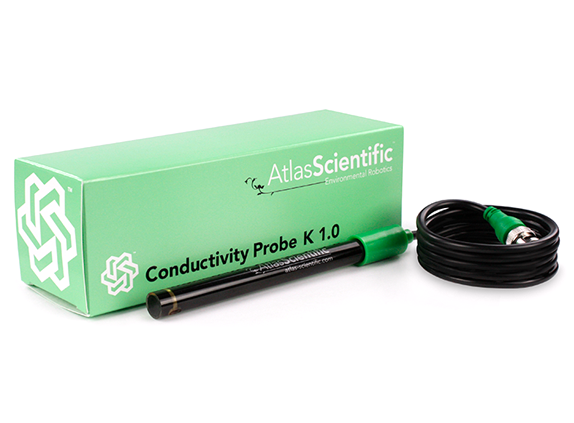
\includegraphics[width=\textwidth]{Imagenes/2021/imag24.png}
        \caption[Sensor de CE]{Sensor de CE.  }
        \label{fig:sensorCE}
     \end{subfigure}
     \hfill
     \begin{subfigure}[b]{0.3\textwidth}
         \centering
         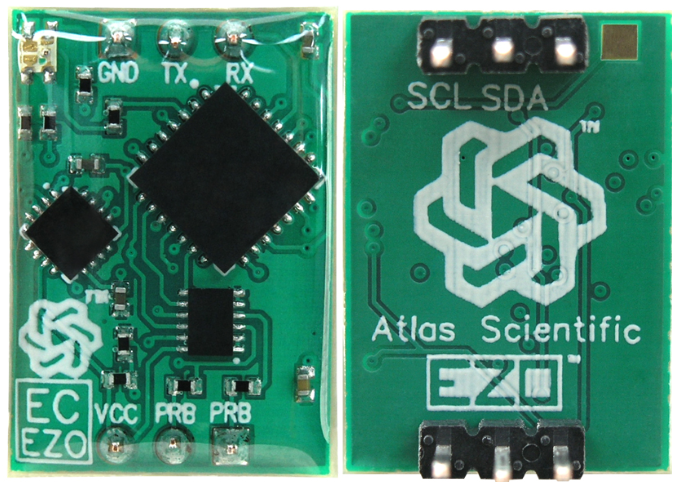
\includegraphics[width=\textwidth]{Imagenes/2021/imag28.png}
        \caption[EZO conductivity Circuit]{EZO conductivity Circuit}
        \label{fig:EZOCE}
     \end{subfigure}
     {\textbf{Fuente:} P\'agina Web del Fabricante\cite{atlasph}.}
     \hfill
\end{figure}

El m\'odulo EZO conductivity circuit, se muestra en la figura \ref{fig:EZOCE} emplea un m\'etodo de resoluci\'on de escala. A medida que aumenta la conductividad, la resoluci\'on entre lecturas disminuye como se puede apreciar en la tabla \ref{tab:resol_ce}.

\begin{table}[t]
    \protect\caption[Resolución de Escala Sensor de Conductividad]{Resolución de Escala Sensor de Conductividad.}\label{tab:resol_ce}
    \centering
    \begin{tabular}{ c r }
    \toprule
    \textbf{Valor}&\textbf{Resolución} \\
          &  $\mu S/cm$ \\
         \midrule
%         \hline
         0.07-99.99 & 0.01  \\
%         \hline
         100.1-999.9 & 0.10 \\
%         \hline
         1,000-9,999 & 1.00 \\
%         \hline
         10,000-99,990 & 10.00 \\
%         \hline
         100,000-999,99 & 100.00  \\
%         \hline
    \bottomrule
    \end{tabular}
    \vspace{5mm}
    \newline
    \textbf{Fuente: }\cite{ezoce}.
\end{table}

\textbf{Principio de operaci\'on: }
Una sonda de conductividad el\'ectrica (CE) mide la conductividad el\'ectrica en una soluci\'on. Se usa com\'unmente en ecosistemas de agua dulce para controlar la cantidad de nutrientes, sales o impurezas en el agua.
Dentro de la sonda de conductividad, dos electrodos se colocan opuestos entre s\'i, como se muestra en la Figura \ref{fig:SensorCEfun}, se aplica un voltaje de CA a los electrodos, lo que hace que los cationes se muevan al electrodo cargado negativamente, mientras que los aniones se mueven al electrodo positivo. Cuanto más electrolito libre contiene el l\'iquido, mayor es la conductividad el\'ectrica.

\begin{figure}[H]
    \centering
    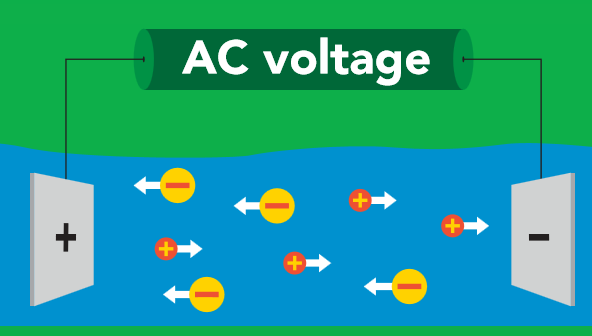
\includegraphics[width=90mm, height=60mm]{Imagenes/2021/imag37.png}
    \caption[Principio de Funcionamiento del Sensor de Conductividad]{Principio de Funcionamiento del Sensor de Conductividad. \textbf{Fuente: }\cite{ezoce}.}
    \label{fig:SensorCEfun}
\end{figure}

En la tabla \ref{tab:caract_ce} se muestran las principales caracter\'isticas del sensor de conductividad.
Entre los usos comunes de este sensor se encuentran el uso est\'andar en laboratorio, uso en el campo, en acuapon\'ia, hidropon\'ia y en acuarios.
\begin{table}[H]
\protect\caption[Caracter\'isticas del sensor de CE de Atlas Scientific]{Caracter\'isticas del sensor de CE de AtlasScientific.}
\label{tab:caract_ce}
\begin{center}
\begin{tabular}{l l}
\hline
Rango    &  5 - 200.000 $\mu S\/cm$\\
Exactitud      &  +/-2\% \\
Conector &  BNC macho\\
Resolución   &  +/-0.0001\\
Tiempo de Respuesta   &  90\% en 1 s\\
Presión Máxima    &  3,447 kPa (500 PSI) \\
Profundidad Máxima	& 343 metros\\
Rango de Temperatura $^{\circ}$C	& 1- 110\\
Longitud del Cable	& 1 m\\
Sensor de Temperatura Interno	& NO\\
Tiempo antes de recalibraci\'on	& 10 año\\
Tiempo de Vida	& aprox. 10 años\\
Dimensiones	& 12 mm x 152 mm\\
Peso	& 51 gramos\\
Superficie de medición	& Grafito\\
Seguro en Alimentos	& Si\\
\hline
\end{tabular}
\vspace{5mm}
\newline
\hfill \textbf{Fuente:} \cite{atlasce}
\end{center}
\end{table}

\subparagraph{Sensor de Temperatura}
En la figura \ref{fig:4.15}  se puede apreciar el sensor de temperatura utilizado fabricado por la empresa Atlas Scientific.

\begin{figure}[ht]
    \centering
    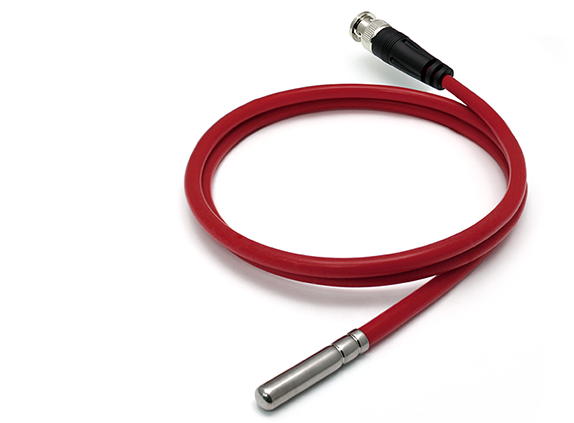
\includegraphics[width=90mm, height=70mm]{Imagenes/2021/imag39.png}
    \caption[Sensor de Temperatura PT 1000]{Sensor de Temperatura PT 1000. }{\textbf{Fuente:} Página Web del Fabricante. }
    \label{fig:4.15}
\end{figure}

\textbf{Principio de funcionamiento:}
A diferencia de cualquier otro material, la correlación entre la resistencia y la temperatura en el platino es bastante lineal. Es por esta razón que el sensor de temperatura RTD de platino es el estándar industrial para la medición de temperatura.
La sonda de temperatura PT-1000 es un term\'ometro tipo resistencia. Donde PT significa platino y 1000 es la resistencia medida de la sonda a 0$^{\circ}$C en $\Omega$ (1k a 0$^{\circ}$C).
A medida que la temperatura cambia, la resistencia del platino cambia.
Para convertir la resistencia de la sonda a la temperatura, se utiliza la siguiente ecuaci\'on simplificada

\begin{equation}
    T=-\frac{\sqrt{(-0.00232(R)+17.59246)}-3.908}{0.00116}
\end{equation}

Donde $T$ est\'a en grados Celsius y $R$ es el valor de la resistencia medida por el sensor.
El módulo utilizado para el tratamiento de las señales es el mostrado en la Figura \ref{fig:4.16} también fabricado por la empresa Atlas Scientific.

\begin{figure}[H]
    \centering
    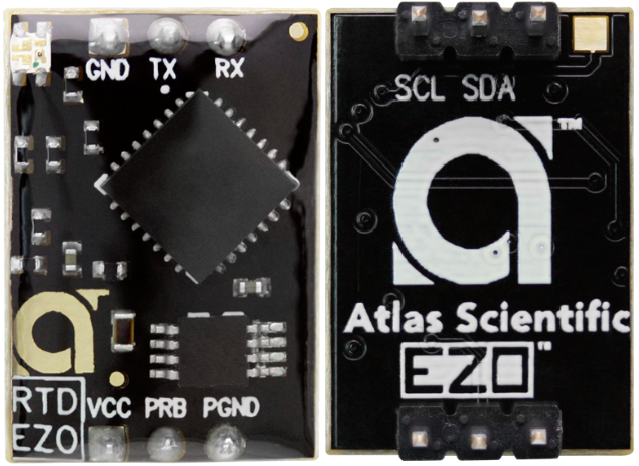
\includegraphics[scale=0.4]{Imagenes/2021/imag38.png}
    \caption[EZO-RTD Circuito Integrado de Temperatura]{EZO-RTD Circuito Integrado de Temperatura.}{\textbf{Fuente:} P\'agina Web del Fabricante.}
    \label{fig:4.16}
\end{figure}

Es un sistema informático de tamaño reducido que está diseñado específicamente para ser utilizado en aplicaciones donde se requiera mediciones exactas y precisas de la temperatura a través de una sonda de temperatura genérica PT-100 / PT-1000. Se conecta directamente a la placa Tentacle T3 y no necesita de aislamiento a diferencia de los otros módulos de sensores.

En la Tabla \ref{tab:caract_temp} se visualizan las características del Sensor de Temperatura PT-1000.
Entre las aplicaciones de uso común de este sensor están el uso est\'andar de laboratorio, uso en el campo, en el suelo, acuapon\'ia, hidroponía, en bebidas como cerveza, vino u otro licor.

\begin{table}[H]
\protect\caption[Características del sensor de temperatura]{Características del sensor de temperatura.}
\label{tab:caract_temp}
\begin{center}
\begin{tabular}{l l}
\hline
Rango    &  -55 $^{\circ}$C a 125 $^{\circ}$C\\
Precisión      &  +/- 0.5 $^{\circ}$C \\
Conector &  BNC macho\\
Tiempo de Respuesta   &  95\% en 1 s\\
Longitud del Cable	& 1 m\\
Tiempo antes de recalibraci\'on	& 1 año\\
Tiempo de Vida	& aprox. 2.5 años\\
Seguro en Alimentos & Si\\
Peso & 49 gramos\\
Dimensiones & 12 mm x 150 mm\\
\hline
\end{tabular}
\vspace{5mm}
\newline
\hfill
\textbf{Fuente: }P\'agina Web del Fabricante,\cite{ezotemp}. 
\end{center}
\end{table} 

\subparagraph{Sensor de OPR/REDOX}
ORP significa potencial de oxidación/reducci\'on, se puede observar en la figura \ref{fig:sensorOPR}, de la empresa Atlas Scientific. La oxidación es la pérdida de electrones y la reducción es la ganancia de electrones. La salida de la sonda se representa en milivoltios y puede ser positivo o negativo.

\begin{figure}[H]
\caption[Sensor y EZO de OPR.]{Sensor y EZO de OPR de la empresa Atlas Scientific. }
     \centering
     \begin{subfigure}[b]{0.5\textwidth}
         \centering
         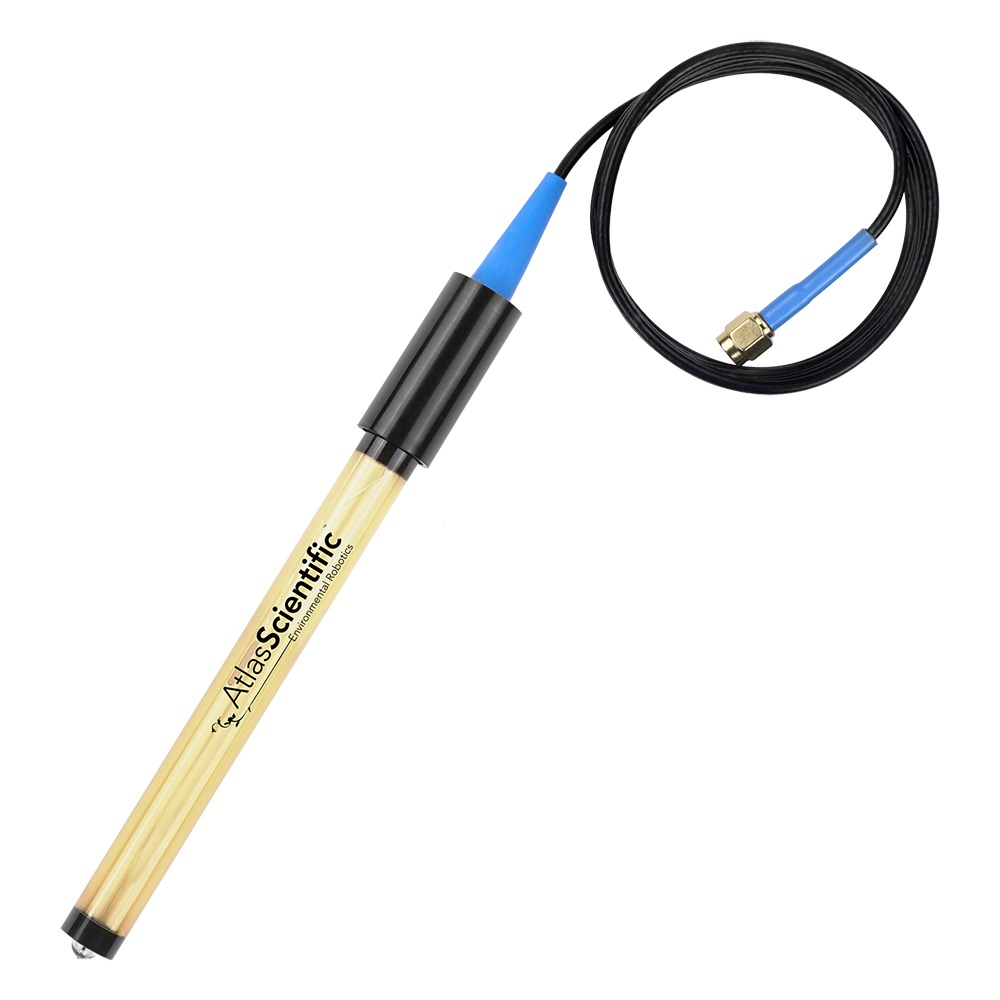
\includegraphics[width=\textwidth]{Imagenes/cap3/OPR_Sensor.jpg}
	    \caption[Sensor de OPR.]{Sensor de OPR . }
        \label{fig:sensorOPR}
     \end{subfigure}
     \hfill
     \begin{subfigure}[b]{0.35\textwidth}
         \centering
         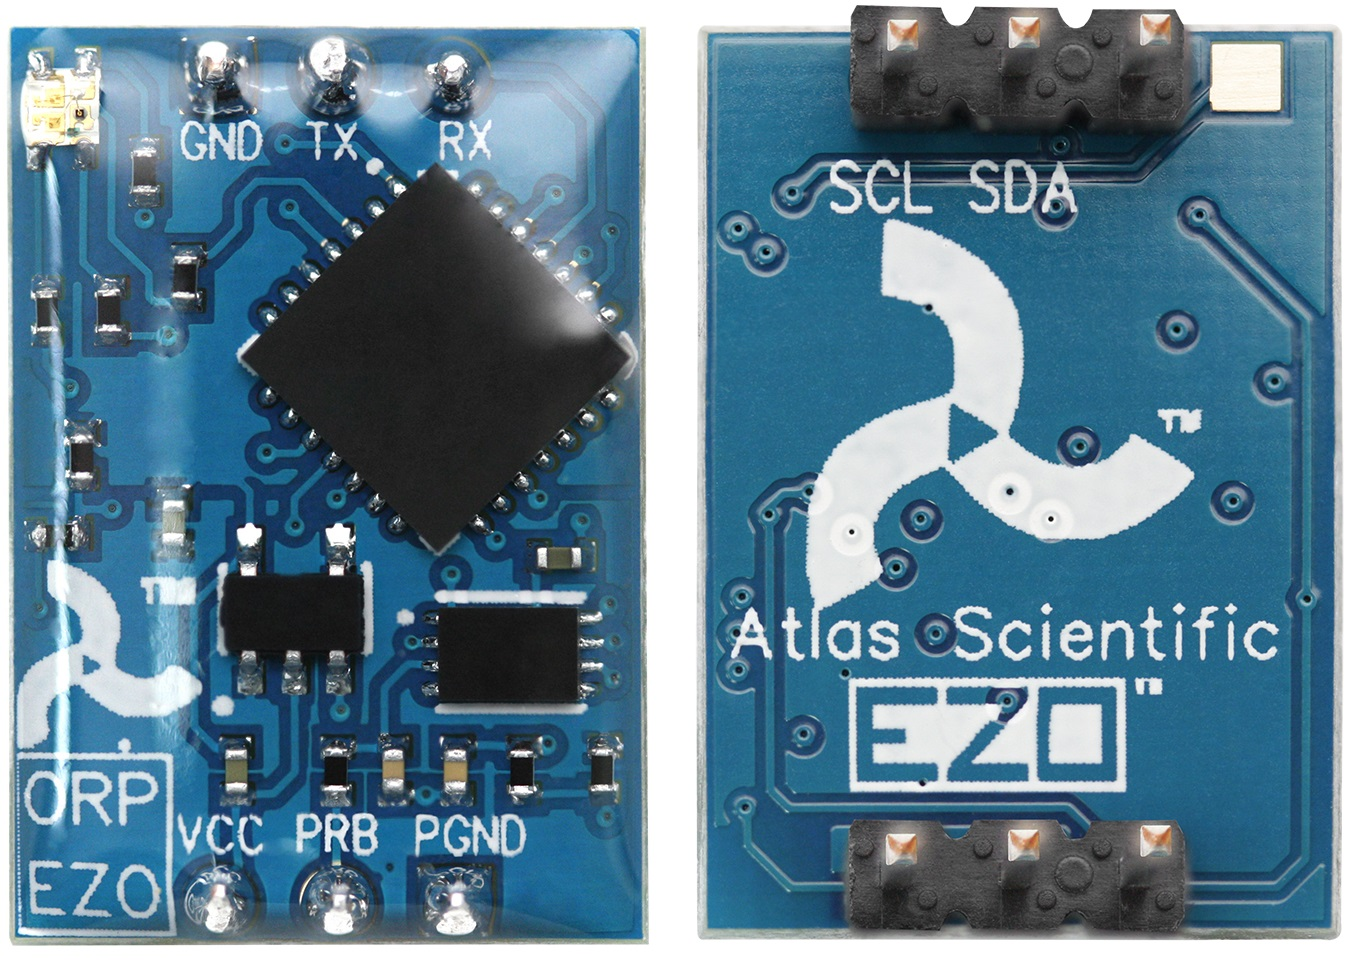
\includegraphics[width=\textwidth]{Imagenes/cap3/OPR_EZO.jpg}
         \caption[EZO OPR Circuit]{EZO OPR Circuit.}
        \label{fig:EZOOPR}
     \end{subfigure}
\textbf{Fuente:} P\'agina Web del Fabricante, \cite{atlas_ezo_OPR}.
     \hfill
\end{figure}

\textbf{Principio de funcionamiento:}
Al igual que una sonda de pH mide la actividad de los iones de hidrógeno en un líquido; una sonda de redox mide la actividad de electrones en un líquido. Las lecturas de ORP representan la fuerza de los electrones transferidos hacia o desde sustancias en un líquido. Teniendo en cuenta que las lecturas no indicar la cantidad de electrones disponibles para la transferencia.
En la figura \ref{fig:OPR_prove} se observa la composición interna de una sonda ORP  tiene una punta de platino que está conectada a un alambre de plata, rodeada con cloruro de plata. Luego, ese cable plateado se conecta a una solución de referencia KCL. Porque platino es un metal no reactivo, puede observar en silencio la actividad electrónica del líquido sin separarse en partes ante cualquier reacción que esté ocurriendo en el líquido.
Una sonda ORP es un dispositivo pasivo que detecta una corriente generada por la oxidación o reducción de sustancias químicas en el agua. Esta corriente (que puede ser positiva o negativa) es muy débil, y no se puede detectar con un multímetro o un convertidor de analógico a digital.
\begin{figure}[H]
    \centering
    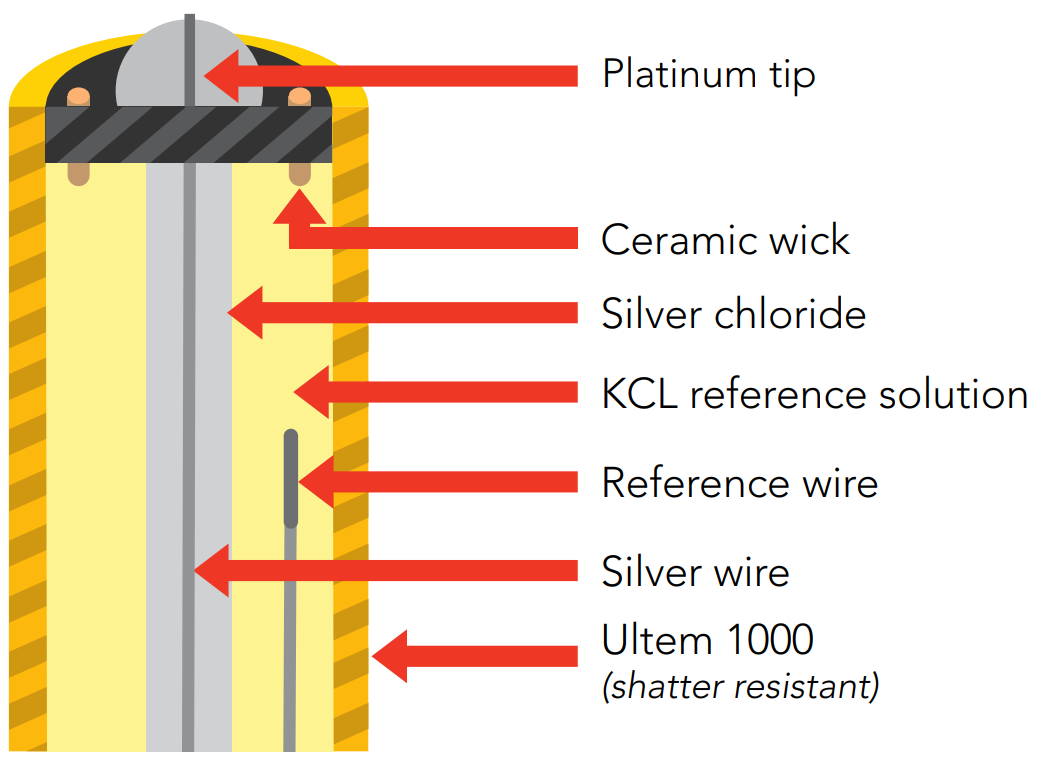
\includegraphics[width=0.5\textwidth]{Imagenes/cap3/sondaOPR.png}
    \caption[Sensor de ox\'igeno disuelto]{Sonda Potencial \'Oxido Reducción.}
    \textbf{Fuente: }P\'agina Web del Fabricante, \cite{atlas_ezo_OPR}.
    \label{fig:OPR_prove}
\end{figure}

En la Tabla \ref{tab:caract_OPR} se muestran las principales características del sensor de conductividad; los usos típicos de este sensor, uso estándar de laboratorio, uso en campo, suelo, muestras que contienen metales pesados, hidroponía, acuaponía, cerveza, vino, alcohol y producción de alimentos.

\begin{table}[H]
\protect\caption[Características del sensor de DO de AtlasScientific]{Características del sensor de DO de AtlasScientific.}
\label{tab:caract_OPR}
\begin{center}
\begin{tabular}{l l}
\hline
Rango   &  +/- 2000     $mV$         \\
Conector &  BNC macho                       \\
Resolución   &  +/- 1 $ mV$              \\
Tiempo de Respuesta   &  95\% en 1s         \\
Presión Máxima    &  689.47 kPa (100 PSI)    \\
Profundidad Máxima	& 60 metros            \\
Rango de Temperatura $^{\circ}$C	& 1- 80\\
Longitud del Cable	& 1 m                    \\
Sensor de Temperatura Interno	& NO        \\
Tiempo antes de recalibración	& aprox. 1 año    \\
Tiempo de Vida	& aprox. 2 años            \\
Dimensiones	& 12 mm x 150 mm                  \\
Peso	& 44 gramos                         \\
Seguro en Alimentos	& Si                    \\
\hline
\end{tabular}
\vspace{5mm}
\newline
\hfill \textbf{Fuente:} P\'agina Web del Fabricante \cite{orp_sensor_measure_nodate}
\end{center}
\end{table}

\subparagraph{Sensor de ox\'igeno disuelto:}
El sensor utilizado para las lecturas de ox\'igeno disuelto se puede apreciar en la figura \ref{fig:sensorDO}, de la empresa Atlas Scientific. La sonda de oxígeno disuelto Atlas Scientific Lab Grade es una sonda pequeña y duradera que puede funcionar en casi cualquier entorno. Desde el trabajo básico de laboratorio hasta el monitoreo remoto. Los criterios de selección fueron su extendido uso para control de calidad de aguas para varios usos, buen soporte y extensa documentación disponible en la web, la homogeneidad en los dispositivos electrónicos. 
El circuito Atlas Scientific EZO-DO, figura \ref{fig:EZODO} le brinda lecturas precisas de OD en Mg/L y porcentaje de saturación. Usando sus funciones de compensación de temperatura, salinidad y presión, puede estar seguro de que las lecturas son correctas sin importar en qué parte del mundo se encuentre. El circuito de oxígeno disuelto EZO de Atlas Scientific es un dispositivo muy sensible. Esta sensibilidad es lo que le da al circuito de oxígeno disuelto su precisión. 

\begin{figure}[H]
\caption[Sensor y EZO de DO.]{Sensor y EZO de DO de la empresa Atlas Scientific. }
     \centering
     \begin{subfigure}[b]{0.5\textwidth}
         \centering
         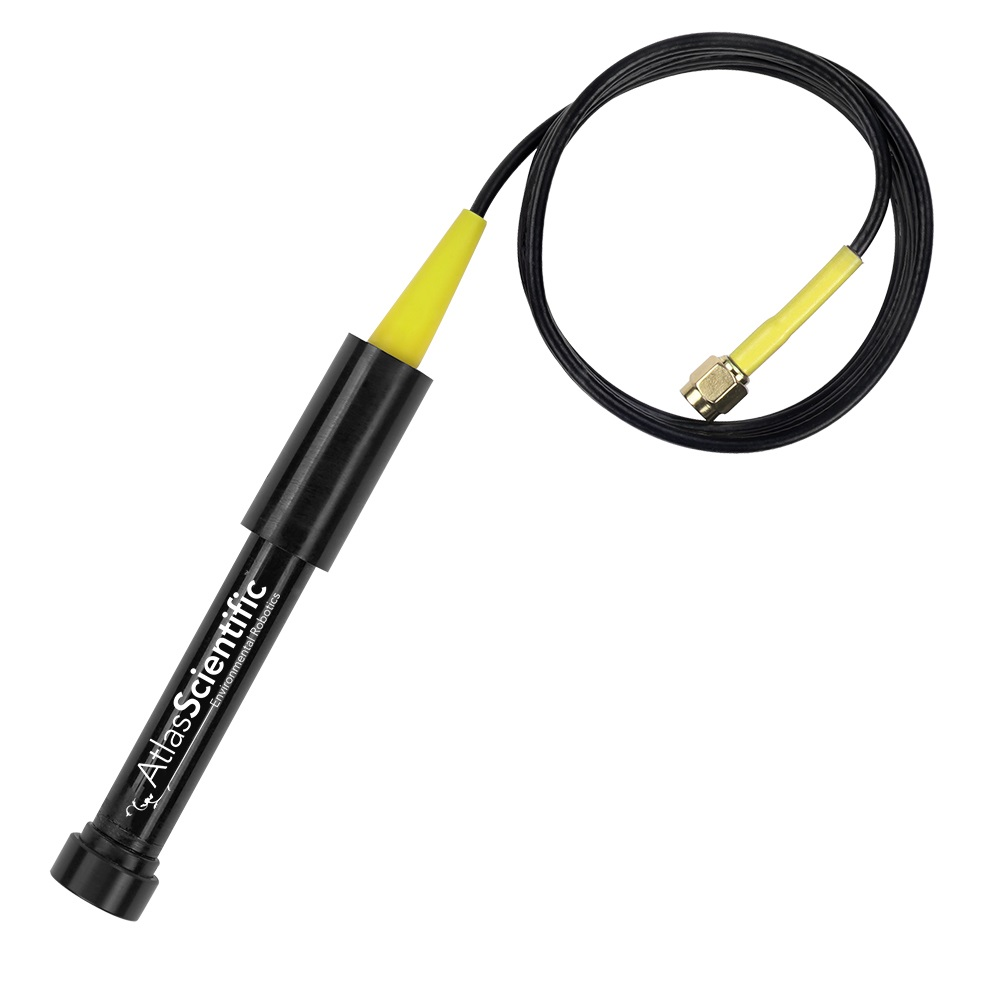
\includegraphics[width=\textwidth]{Imagenes/cap3/OD_Sensor.jpg}
	    \caption[Sensor de DO.]{Sensor de DO . }
        \label{fig:sensorDO}
     \end{subfigure}
     \hfill
     \begin{subfigure}[b]{0.35\textwidth}
         \centering
         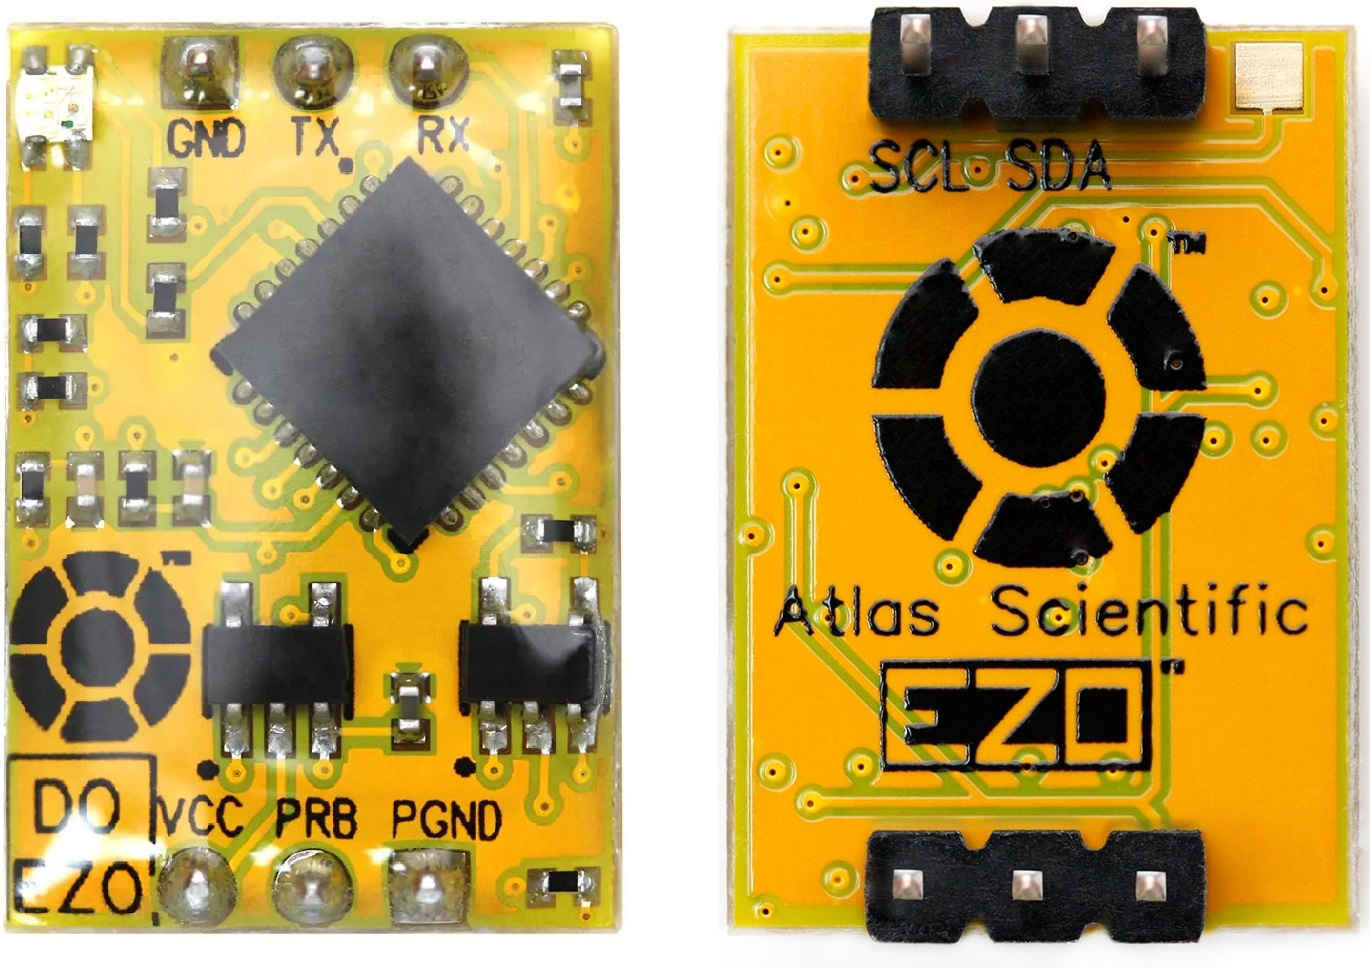
\includegraphics[width=\textwidth]{Imagenes/cap3/EZO_DO.jpg}
         \caption[EZO DO Circuit]{EZO DO Circuit.}
        \label{fig:EZODO}
     \end{subfigure}
\textbf{Fuente:}P\'agina Web del Fabricante,\cite{atlas_dissolved_DO}.
\hfill
\end{figure}

\textbf{Principio de funcionamiento:} Una sonda galv\'anica de ox\'geno disuelto consta de una membrana de politetra fluoroetileno (PTFE), un \'anodo ba\~nado en un electrolito y un c\'atodo figura \ref{fig:DO_prove}.
Las mol\'eculas de ox\'igeno se desactivan a trav\'es de la membrana de la sonda a una velocidad constante (sin la membrana, la reacci\'on es demasiado r\'apida). Una vez que las mol\'eculas de ox\'igeno han atravesado la membrana, se reducen en el c\'atodo y se produce un peque\~no voltaje. Si no hay mol\'eculas de ox\'igeno presentes, la sonda emitir\'a 0 mV. A medida que aumenta el oxígeno, también lo hace la salida de mV de la sonda. Cada sonda emitirá un voltaje diferente en presencia de oxígeno. Lo único que es constante es que 0 mV = 0 Oxígeno

\begin{figure}[H]
    \centering
    % 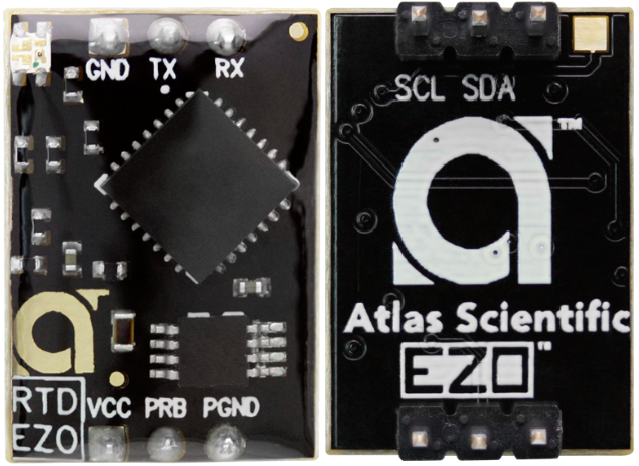
\includegraphics[width=90mm, height=70mm]{Imagenes/2021/imag38.png}
    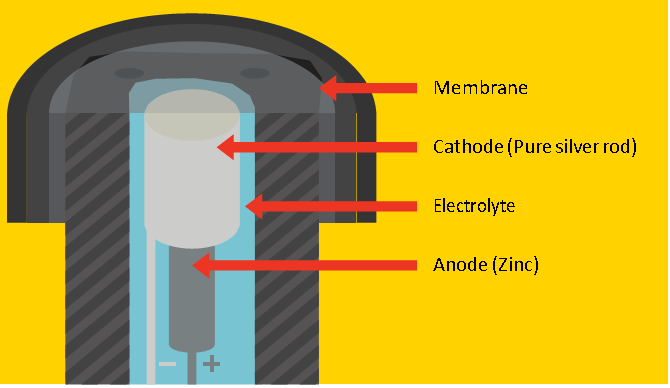
\includegraphics[scale=1.5]{Imagenes/cap3/DO.png}
    \caption[Sensor de ox\'igeno disuelto]{Sonda ox\'igeno disuelto.}{\textbf{Fuente:} P\'agina Web del Fabricante,\cite{atlas_scientific_lab_nodate}.}
    \label{fig:DO_prove}
\end{figure}

En la Tabla \ref{tab:caract_do} se muestran las principales caracter\'isticas del sensor de conductividad. Los usos t\'ipicos de este sensor son cultivos hidrop\'onicos, piscicultura, monitoreo ambiental, elaboraci\'on de vino.

\begin{table}[H]
\protect\caption[Caracter\'isticas del sensor de DO de Atlas Scientific]{Caracter\'isticas del sensor de DO de Atlas Scientific.}
\label{tab:caract_do}
\begin{center}
\begin{tabular}{l l}
\hline
Rango   &  0.01 - 100     $mg/L$         \\
Conector &  BNC macho                       \\
Resolución   &  +/-      0.05 $ mg/L$              \\
Tiempo de Respuesta   &  90\% en 1 s         \\
Presión Máxima    &  3,447 kPa (500 PSI)    \\
Profundidad Máxima	& 343 metros            \\
Rango de Temperatura $^{\circ}$C	& 1- 50\\
Longitud del Cable	& 1 m                    \\
Sensor de Temperatura Interno	& NO        \\
Tiempo antes de recalibración	& aprox. 1 año    \\
Tiempo de Vida	& aprox. 5 años            \\
Dimensiones	& 16.57 mm x 114 mm                  \\
Peso	& 52 gramos                         \\
Tipo de membrana	& Tefl\'on           \\
Seguro en Alimentos	& Si                    \\
\hline
\end{tabular}
\vspace{5mm}
\newline
\hfill \textbf{Fuente:} \cite{atlas_dissolved_DO}
\end{center}
\end{table}

\textbf{Bloque de Control}
Este bloque es el encargado de realizar el procesamiento de los datos recibidos a través de los sensores y la configuración de parámetros adquirida por la Interfaz de Usuario.

\begin{itemize}
    \item \textbf{Hardware:}
    En la Figura \ref{fig:raspberry} se observa la placa de desarrollo low cost escogida para el presente proyecto, la Raspberry Pi 3 model B desarrollado por la fundación Raspberry Pi. La misma cuenta con un procesador multimedia Broadcom BCM2835 system-on-chip (SoC).
    La CPU Contiene un ARM1176JZFS, con unidad de coma flotante, que funciona a 700 Mhz y es capaz de soportar overclock a 1 GHZ en modo “TURBO” que hace que el SoC de más rendimiento sin reducir el tiempo de vida de la placa y sin perder la garantía. 
    La memoria RAM es de 512 MB de SDRAM (en su modelo B), en un único módulo, el cual, funciona a 400 Mhz en su modo normal y alcanzando los 600 Mhz en su versión “TURBO”.
    La  Raspberry Pi no tiene un disco duro tradicional, para ello dispone de un lector para memorias SD, un sistema de almacenamiento en estado sólido. El arranque del sistema se hará desde la propia tarjeta SD, con lo que, debido a que tiene que albergar todo el sistema operativo, es necesario que la tarjeta sea de al menos 2 GB de capacidad para almacenar todos los archivos requeridos.
    La placa carece de botón de encendido y apagado, con lo que la energía le llega mediante un conector microUSB estándar de 5 V. El consumo de la placa es de 700 mA, (3,5 W).
    La Raspberry Pi, está diseñada para ejecutar el sistema operativo GNU/Linux y la versi\'on m\'as extendido es el Raspberry Pi OS.
    
\begin{figure}[H]
\centering
     \begin{subfigure}[b]{0.45\textwidth}
         \centering
         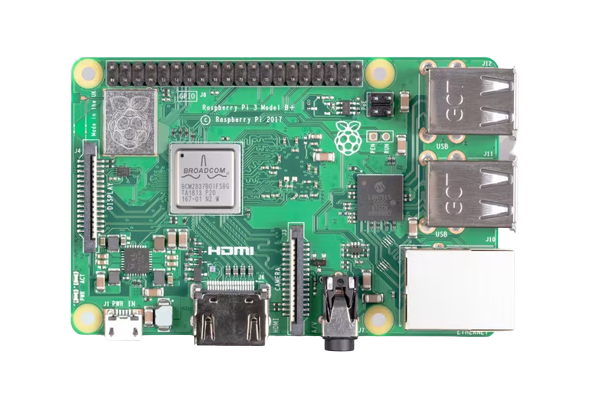
\includegraphics[width=\textwidth]{Imagenes/cap3/raspberry_1.png}
     \end{subfigure}
\hfill
     \begin{subfigure}[b]{0.45\textwidth}
         \centering
         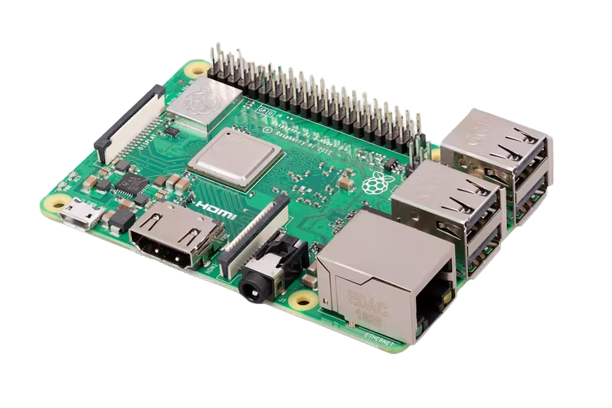
\includegraphics[width=\textwidth]{Imagenes/cap3/raspberry_2.png}
     \end{subfigure}
\caption[Placa Raspberry Pi 3 model B]{Placa Raspberry Pi 3 model B.}
\textbf{Fuente:}P\'agina Web del Fabricante\cite{atlas_dissolved_DO}
\label{fig:raspberry}
\hfill
\end{figure}

Se opt\'o por este computador de un chip por sus prestaciones,  t\'ecnicas, suficientes para las tareas a ser ejecutadas, con un almacenamiento externa de 64 Gb con una memoria tipo microSD de alto rendimiento, por sus dimensiones reducidas, la raspberry pi eran acorde a los requerimientos necesarios y por tener un gran soporte y comunidad activa en l\'inea.
En la Tabla \ref{tab:carac_rasp} se detallan las principales características técnicas de la Raspberry Pi 3 model B.
 \begin{table}[t]
      \protect\caption[Características Técnicas. Raspberry Pi 3 model B]{Características Técnicas. Raspberry Pi 3 model B.  \label{tab:carac_rasp}}
     \centering
     \begin{tabular}{l c}
        \toprule
           Sistema Operativo & Raspberry Pi OS\\
%          \hline
          Juego de Instrucciones & RISC 64 bits\\
%          \hline
          Procesador & RQuad Core 1,2 GHz Broadcom BCM2837\\
%          \hline
          RAM  & 1 GB\\
%          \hline
          Bluetooth &  4.2 Low Energy (BLE)\\
%          \hline
          Puertos USB 2.0 & 4\\
%          \hline
          GPIO& 40\\
%          \hline
          UART& 2\\
%          \hline
          I2C& 4\\
%          \hline
          Stero/Video & 1\\
%          \hline
          HDMI & 1\\
%          \hline
          CSI(RPI Camera) & 1\\
%          \hline
          DSI(RSP Touchscreen display) & 1\\
%          \hline
          Dimensiones & 85.60 mm x 53.98 mm\\
%          \hline
          Peso & 50 g\\
%          \hline
          Consumo energ\'etico & 3.5 W\\
%          \hline
          Alimentaci\'on & 5 V\\
%          \hline
     \bottomrule   
     \end{tabular}
     \vspace{5mm}
     \newline
     \hfill \textbf{Fuente:} Elaboración Propia. Información recopilada de \cite{rasp}
\end{table}
    Por otra parte, para eliminar la necesidad de cableado, multiplexación y aislamiento eléctrico en la lectura de los sensores, se optó por la utilización de la placa open source Tentacle Shield para arduino de Whitebox labs, la cual se muestra en la Figura \ref{fig:4.5}.
\begin{figure}[ht]
    \centering
    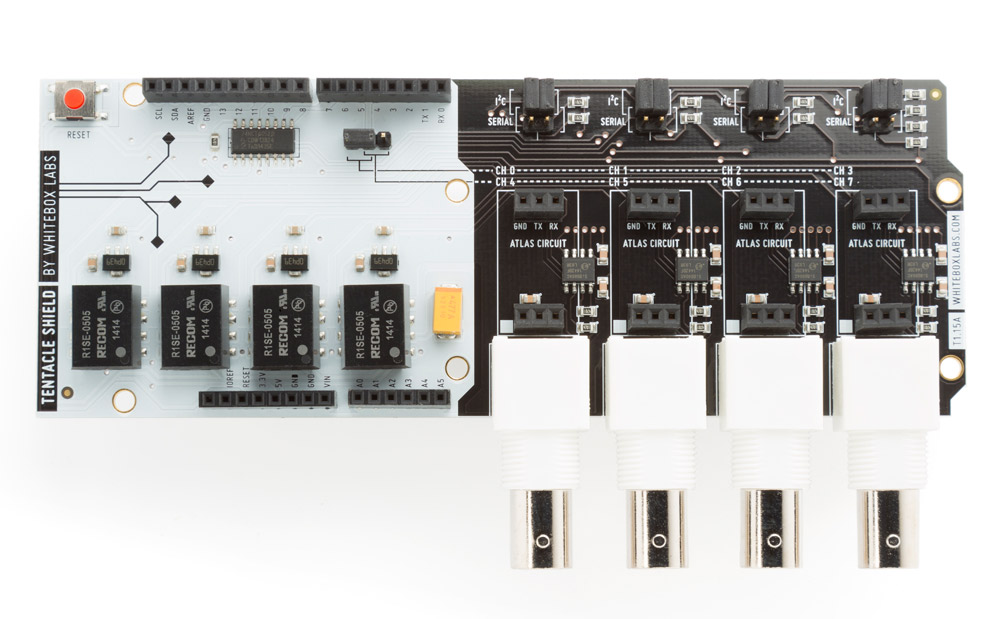
\includegraphics[width=0.7\linewidth]{{Imagenes/2021/imag26.jpg}}
    \caption[Placa Tentacle para Arduino]{Placa Tentacle para Arduino. }{\textbf{Fuente:} Página web del Fabricante,\cite{whiteboxes-no-date}}
    \label{fig:4.5}
\end{figure}
    Es una forma pr\'actica y fácil de leer múltiples sensores de la empresa Atlas Scientific, la placa puede alojar hasta 4 dispositivos EZO de Atlas Scientific para medir pH(Potencial de Hidrógeno), Oxígeno Disuelto(DO por sus siglas en inglés), conductividad eléctrica(CE), Temperatura(T), Potencial de Reducción de Oxidación(ORP por sus siglas en inglés)
    \textbf{Aislamiento:}
    Los circuitos de medición y las líneas de comunicación aislados individualmente evitan el ruido y los bucles de tierra para obtener mediciones precisas, incluso en sistemas de bucle cerrado. Los sensores no interferirán entre sí y la mayoría del ruido eléctrico exterior que puede interferir con las lecturas se reducirá.
    \item \textbf{Software:}El software de control fue desarrollado en el lenguaje de programación Python. Este es un lenguaje interpretado multiparadigma, soporta programación orientada a objetos, imperativa y funcional.
    Python ya viene instalado en el sistema operativo Raspberry Pi OS para Raspberry Pi. Tiene la ventaja de poder utilizar los pines GPIO de la placa de desarrollo para conectar el mundo digital con el mundo físico mediante la programación, facilitando de esta manera el control de la lectura de los distintos sensores y el accionamiento de los actuadores utilizados.
    El administrador de Base de Datos utilizado fue Sqlite3, es un sistema de gestión de base de datos ampliamente difundido en el mundo de la programación de aplicaciones móviles.
    La utilización de este gestor fue debido a su gran portabilidad y su capacidad  de gestionar bases de datos de hasta 2 terabytes de tamaño.
    En la Tabla \ref{tab:caract_sqlite} se muestran las características más relevantes de la Base de Datos Sqlite.
    
    \begin{table}[H]
    \protect\caption[Características del Gestor de Base de Datos SQLITE]{Características del Gestor de Base de Datos SQLITE.
    \label{tab:caract_sqlite}}
        \centering
        \begin{tabular}{l l}\\ \midrule
            Soporte & Múltiples tablas,\textit{triggers} y vistas   \\
            
             Lectura y Escritura& \multicolumn{1}{l}{\begin{tabular}[c]{@{}l@{}}  Directamente sobre archivos que se\\ encuentran en el disco  duro.\end{tabular}} 
             \\
             Formato & 
             \multicolumn{1}{l}{\begin{tabular}[c]{@{}l@{}}  Multiplataforma. Puede ser utilizado \\en sistemas de 32 bits \\ o 64 bits.\end{tabular}} 
           \\
             Operaciones &\multicolumn{1}{l}{\begin{tabular}[c]{@{}l@{}} Realiza operaciones de manera más\\ eficiente y rápido que  \\ MySql y PostgreSQL.\end{tabular}} 
            \\
             Interfaz API &\multicolumn{1}{l}{\begin{tabular}[c]{@{}l@{}}Opera con diversas Interfaces API \\lo que permite trabajar  \\con C++, PHP, Python, Groovy, etc.\end{tabular}} 
            \\
            Dependencias Externas & No\\
    
             Librerías & Cuentan con acceso para muchos\\ lenguajes de programación.\\
    
             UDF & Soporta funciones SQL definidas por el usuario.\\

             Código Fuente & Dominio público y documentación extensa.\\
             \hline
        \end{tabular}
        \vspace{5mm}
        \newline
        \hfill \textbf{Fuente: }P\'agina Web del desarrollador,\cite{sqlite}.
    \end{table}
\end{itemize}

A continuaci\'on, en la tabla \ref{tab:tablasBD}, se presenta el dise\~no f\'isico de la base de datos:

% Please add the following required packages to your document preamble:
% \usepackage{booktabs}
\begin{table}[H]
\centering
\caption{Dise\~no f\'isico de la base de datos}
\label{tab:tablasBD}
\begin{tabular}{@{}llc@{}}
\toprule
\multicolumn{3}{c}{Tabla muestreo}                        \\ 
Atributo       & Descripci\'on               & Tipo de dato \\ \midrule
idMuetreo (PK) & index de muestreo         & INTEGER      \\
dataTime       & Fecha y hora              & TEXTO        \\
Temp           & Temperatura               & REAL         \\
pH             & Potencial de hidr\'ogeno    & REAL         \\
DO             & Ox\'igeno disuelto          & REAL         \\
CE             & Conductividad el\'ectrica   & REAL         \\
TDS            & Total solidos disueltos   & REAL         \\
S              & Salinidad                 & REAL         \\
OPR            & Potencial \'oxido reducci\'on & REAL         \\ \bottomrule
\end{tabular}
\end{table}

%% Fabricacion
La fabricaci\'on de la sonda requiri\'o de varios tipos de procesos de mecanizado, de acuerdo a las caracter\'isticas de cada una de sus partes, por un lado, el cuerpo principal de la sonda compuesto por los m\'odulos de la base y el m\'odulo del anillo, los m\'odulos más cr\'iticos por contener todo el sistema electr\'onico, el\'ectrico y comunicaci\'on, es indispensable ser totalmente herm\'etico, para impedir que el agua ingrese a la sonda, por ese motivo se determin\'o, que deb\'ia ser mecanizado a partir de una pieza r\'igida, para la selecci\'on del material de la pieza rígida, se tuvieron en cuenta tres materiales, acero inoxidable, acero aleado y tefl\'on, principalmente por su disponibilidad en el mercado paraguayo, y propiedad de resistencia a la oxiadaci\'on, ya que estar\'a expuesto por estar en contacto constante con el agua. 
Los materiales met\'alicos quedaron descartados por ser elementos atenuantes de se\~nales inal\'ambricas como ser sen\~nal wifi, perif\'erico de rat\'on y teclado inal\'ambrico, bluetooth entre otros. Otro factor que se tuvo en cuenta para la selecci\'on del material fue su costo de adquisici\'on  y proceso de mecanizado m\'as especializado, en cambio, la opción no met\'alica consideradas del tipo tefl\'on, satisface las caracterí\'isticas mec\'anica y el\'ectricas proyecto, tal como se puede observar en la tabla. 
El tefl\'on o el politetrafluoretileno (PTFE), pertenece a la familia de los pol\'imeros, llamados fluoropol\'imeros. El PTFE es resistente en extremo al ataque qu\'imico y ambiental, no le afecta el agua, posee buenas propiedades el\'ectricas, buena resistencia al calor y coeficiente de fricci\'on muy bajo, \cite{groover_fundamentos_1997}.
Seleccionado el material, por su presentaci\'on de tubo r\'igido, se opt\'o por la t\'ecnica de fabricaci\'on sustractiva para la fabricaci\'on de los modulos base y anillo, consistente en la remoci\'on o frezado de materiales pieza r\'igida, a modo de lograr un vaciado interno de la pieza hasta lograr el dise\~no deseado, este proceso de fabricaci\'on se llev\'o a cabo en el laboratorio de metal mec\'anica de FIUNA, tal como se observa en la figura \ref{fig:preparacion}.

\begin{figure}[H]
\centering
     \begin{subfigure}[b]{0.45\textwidth}
         \centering
         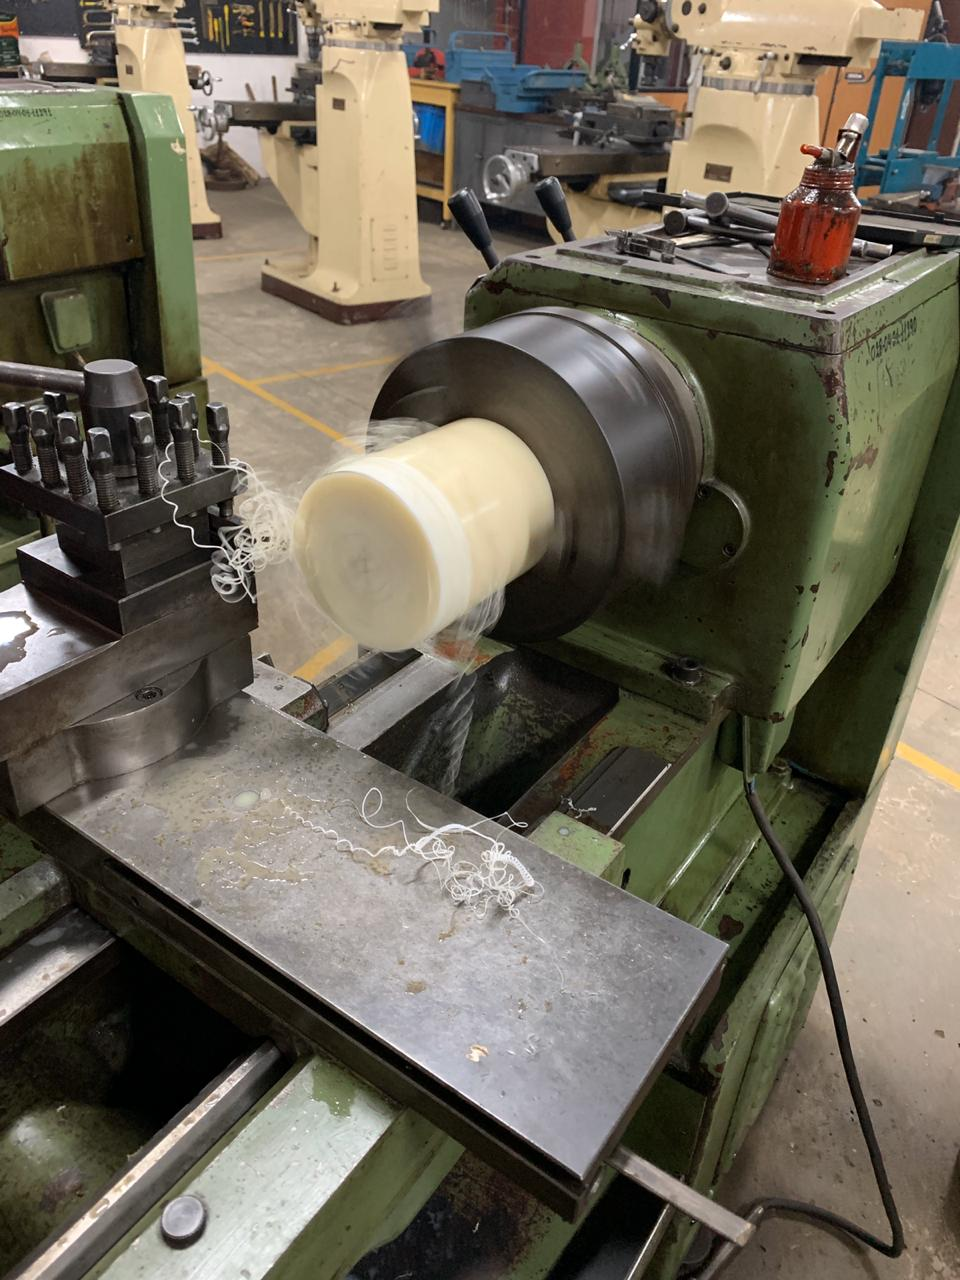
\includegraphics[width=0.7\textwidth]{Imagenes/2019/Sonda_Fab0.jpeg}
         \caption{Proceso de desgaste.}
         \label{fig:preparacion}
     \end{subfigure}
     \begin{subfigure}[b]{0.5\textwidth}
         \centering
         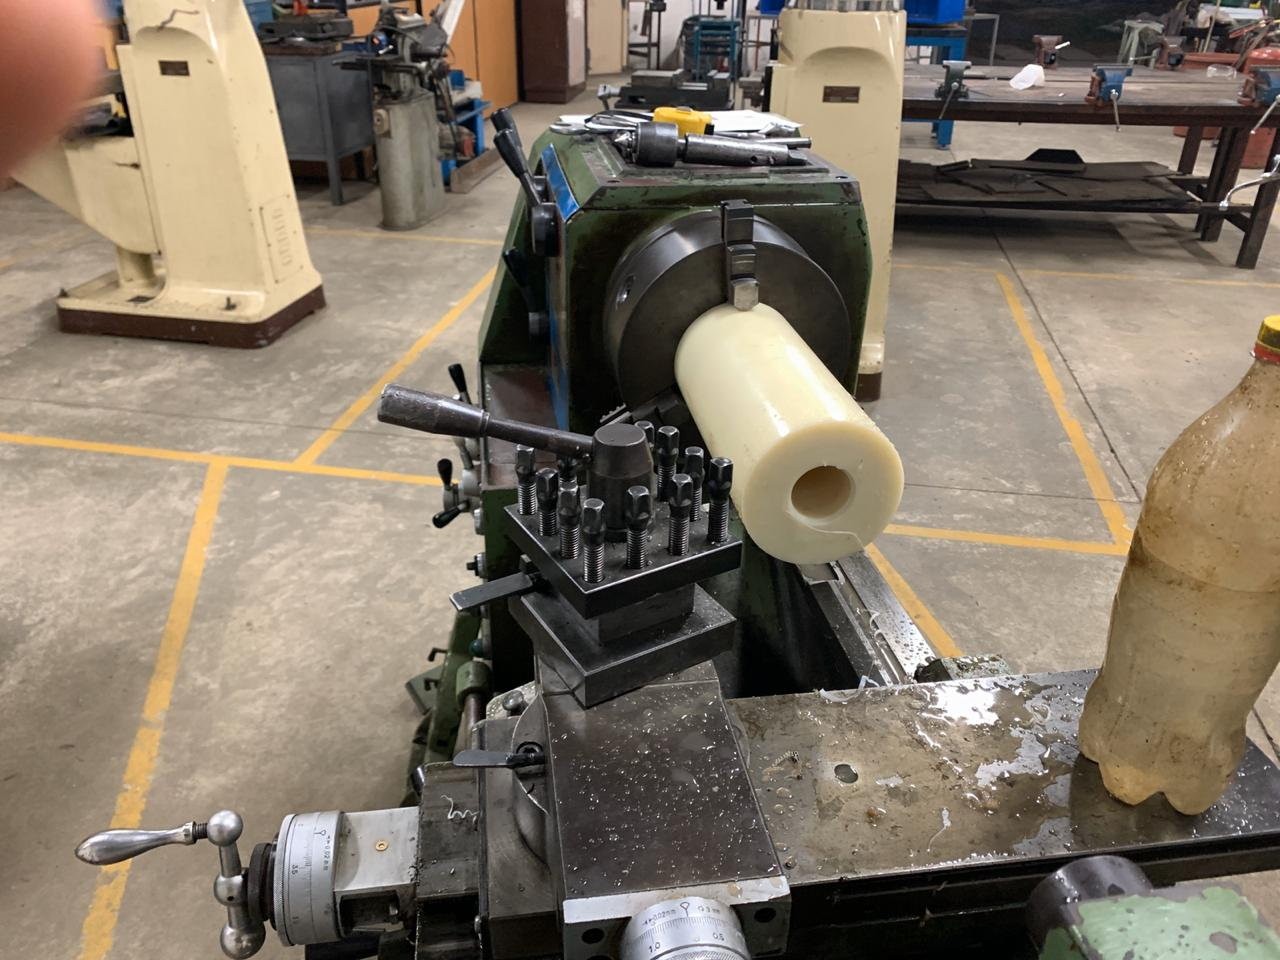
\includegraphics[width=\textwidth]{Imagenes/2019/Sonda_Fab.jpeg}
         \caption{Proceso de vaciado}
         \label{fig:preparacion_vaciado}
     \end{subfigure}
\caption[Proceso de mecanizado. Tubo de tefl\'on]{Proceso de mecanizado.}
\textbf{Fuente:}Elaboraci\'on propia.
\hfill
\end{figure}

El procedimiento fue realizado por los encargados del laboratorio con un torno semi autom\'atico, se procedi\'o al vaciado progresivo de la pieza siguiendo una secuencia de operaciones descritas a continuaci\'on.

\begin{enumerate}
\renewcommand{\theenumi}{\alph{enumi}} %Letras minúsculas
     \item Careado: a la primera operaci\'on realizada por torno fue el careado a tal forma de nivelar, limpiar toda la superficie, dejando una superficie totalmente plana, consistente en una herramienta operada por el operario que lo sit\'ua radialmente sobre el extremo del trabajo rotatorio. Fig.\ref{fig:torneado}(a).
    \item Tronzado: segunda opraci\'on realizado, consisti\'o en el tronzado de la pieza a fin de lograr obtener una superficie de trabajo limpia y uniforme, la herramienta manejada por el operario avanza radialmente en la cara de forma conc\'entrica en el sentido de rotaci\'on, a lo largo de su di\'ametro. Fig.\ref{fig:torneado}(b) 
    \item Taladrado: como el volumen  a ser removido superaba el 80 {\%} de la pieza, se requirió un avance progresivo mediante dos brocas, donde el operador hace avanzar la broca dentro del \'area de trabajo rotatorio a lo largo de todo su eje, con esto se conseguir\'a ir incrementando progresivamente la abertura para el siguiente proceso. Fig.\ref{fig:torneado}(c)
    \item Perforado: Una herramienta de punta sencilla avanza en línea paralela al eje de rotación, sobre el diámetro interno de un agujero existente en la pieza. Fig.\ref{fig:torneado}(d)
    \item Roscado: Una herramienta puntiaguda avanza linealmente a través de la superficie externa de la pieza de trabajo en rotación y en dirección paralela al eje de rotación, a una velocidad de avance suficiente para crear cuerdas roscadas en el cilindro. Fig.\ref{fig:torneado}(e)
\end{enumerate}

\begin{figure}[H]
\centering
\fbox{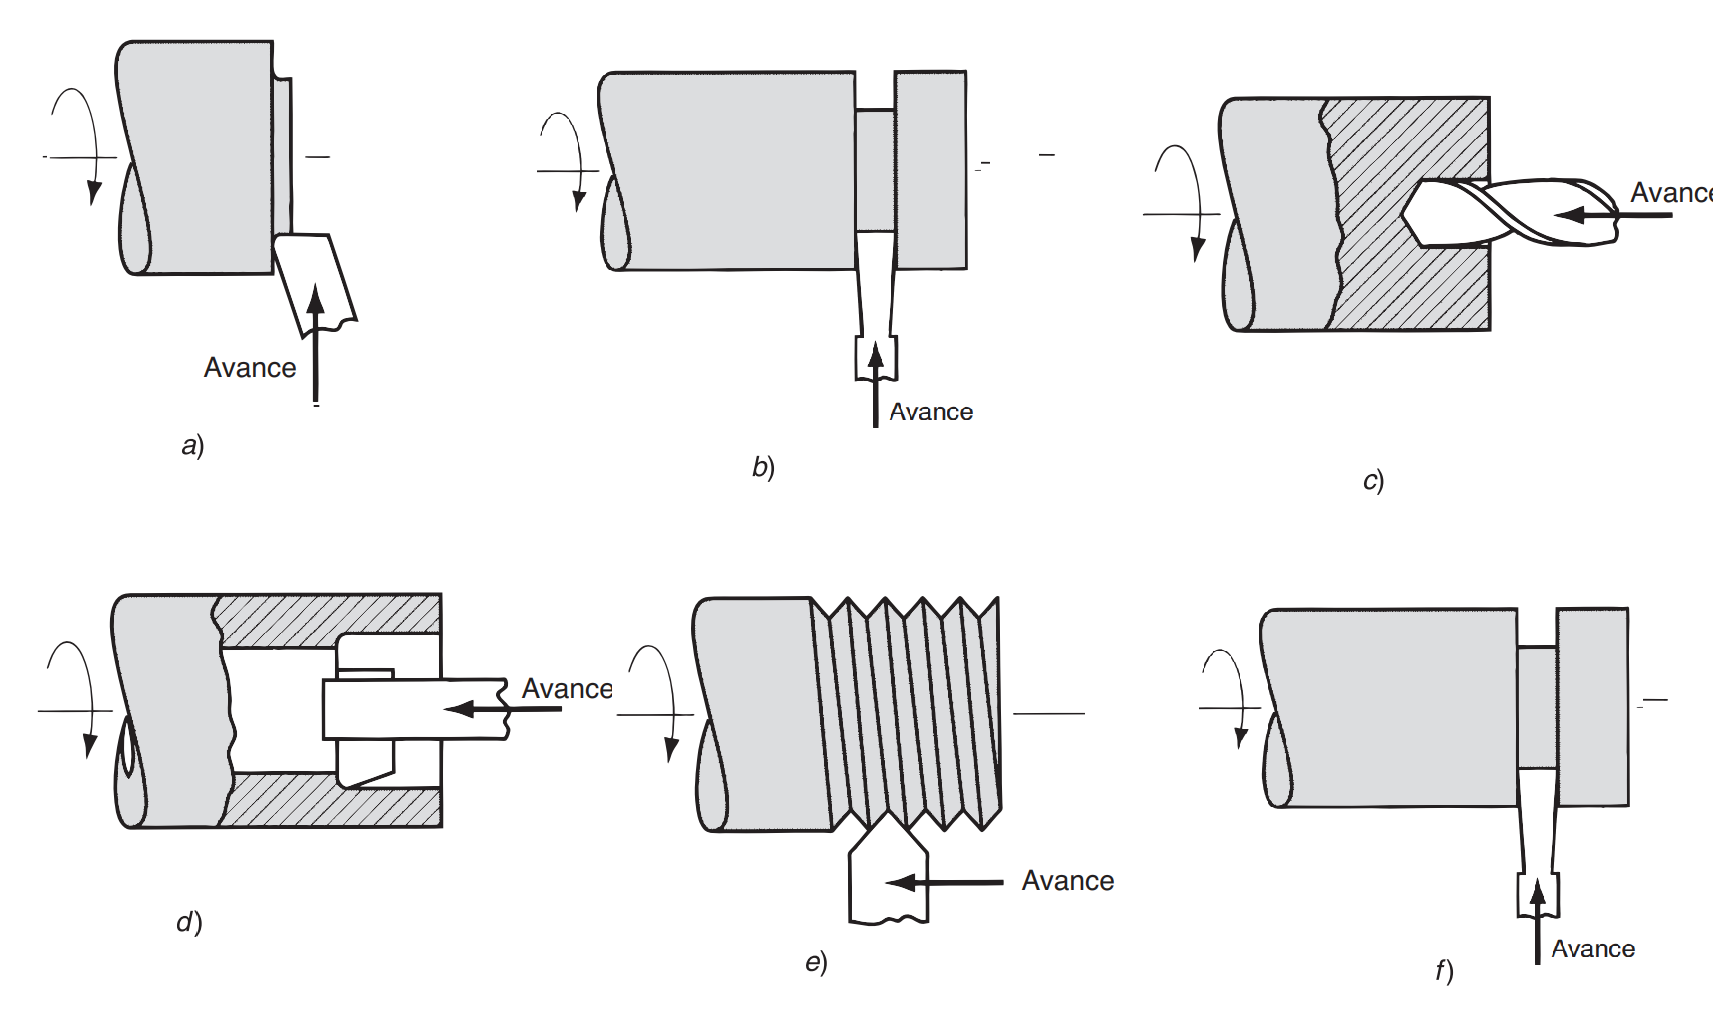
\includegraphics[scale=0.7]{Imagenes/cap3/mecanizado.png} }
\caption{Secuencia de operaciones}{\textbf{Fuente:} Fundamentos de manufactura moderna, \cite{groover_fundamentos_1997}}.
\label{fig:torneado}
\end{figure}

Para asegurar que el peso del la sonda pueda ser sumergida, se considera el principio del Arqu\'imedes, cuando tiramos un objeto al agua; el objeto se hunde si su peso es mayor que el peso del fluido desalojado (desplazado). El objeto flota cuando su peso es menor o igual al peso del fluido desplazado. 
Para el c\'alculo del peso extra que debe ser agregado a la sonda para que pueda sumergir.

\begin{equation}
E=\rho_{liq}*g*V_{cuerpo} 
\label{eq:empuje}
\end{equation}
v=0.00745264 $m^3$

$\rho_{liq}$= Densidad del l\'iquido.
$V_{cuerpo}$ = volumen del cuerpo.
$g$ = gravedad

Reemplazando los valores en la f\'ormula \ref{eq:empuje}, tenemos
$$ \rho_{liq} = 1 \frac{g}{cm^{3}}$$  
$$ g= 981 \frac{cm}{s^{2}}$$
$$ V_{cuerpo}= \pi * (30*12.5^{2}-20*10.5^{2})= 7452.64 cm^{3}$$
$$ E= 1 * 7452.64 * 981 = 7311039.84 \textit{[dina]} = 73.11 \textit{[N]}$$

Para que se pueda sumergir el peso debe de ser mayor a al empuje E.
\begin{equation}
m_{cuerpo} * g > E 
\label{eq:empuje2}
\end{equation}
$m >\frac{E}{g}$
$m > 73.11/9.81$
$m > 7.45 [Kg] $, el cual ser\'a agregado en formato de pesos extra a la sonda.

\section{Medidor de profundidad}
Este subsistema auxiliar, está pensado por la capacidad de medici\'on a multi niveles, cuando se requiera que la sonda descienda el subsistema se encargara de censar la profundidad en el punto de descenso y mandar la informaci\'on a la sonda para seteo de la carrera de la gr\'ua. Se opt\'o por una estructura simple, de bajo costo,  modular y vers\'atil para varios modos de uso.  
Tal como se observa en la figura \ref{fig:batimetro} el sistema de medici\'on de profundidad fue dise\~nado de tal forma que permita ser instalado en la parte posterior (popa) del VAS, mediante dos abrazaderas, uno de su sujeci\'on y otra de sujeci\'on - nivelaci\'on para asegurarse  pueda estar en contacto con el agua al momento de instalarse.  Para la correcta  instalaci\'on de se debe alinear el sonar con la parte m\'as baja de la popa para estructura del sistema de batimetr\'ia tubos de PVC (Policloruro de Vinilo) roscables para la construcci\'on de la estructura de soporte, la secci\'on m\'as larga tiene una longitud de 1,5 [m], con el objetivo de poder ajustar la distancia de medici\'on inicial y que el sonar ubicado en el extremo est\'e totalmente sumergido. El sistema de fijaci\'on y ajuste est\'a compuesta por dos abrazaderas, una del tipo omega utilizada como gu\'ia de desplazamiento y la otra de abrazadora tipo anillo para el ajuste de profundidad. 
\begin{figure}[H]
\centering
\fbox{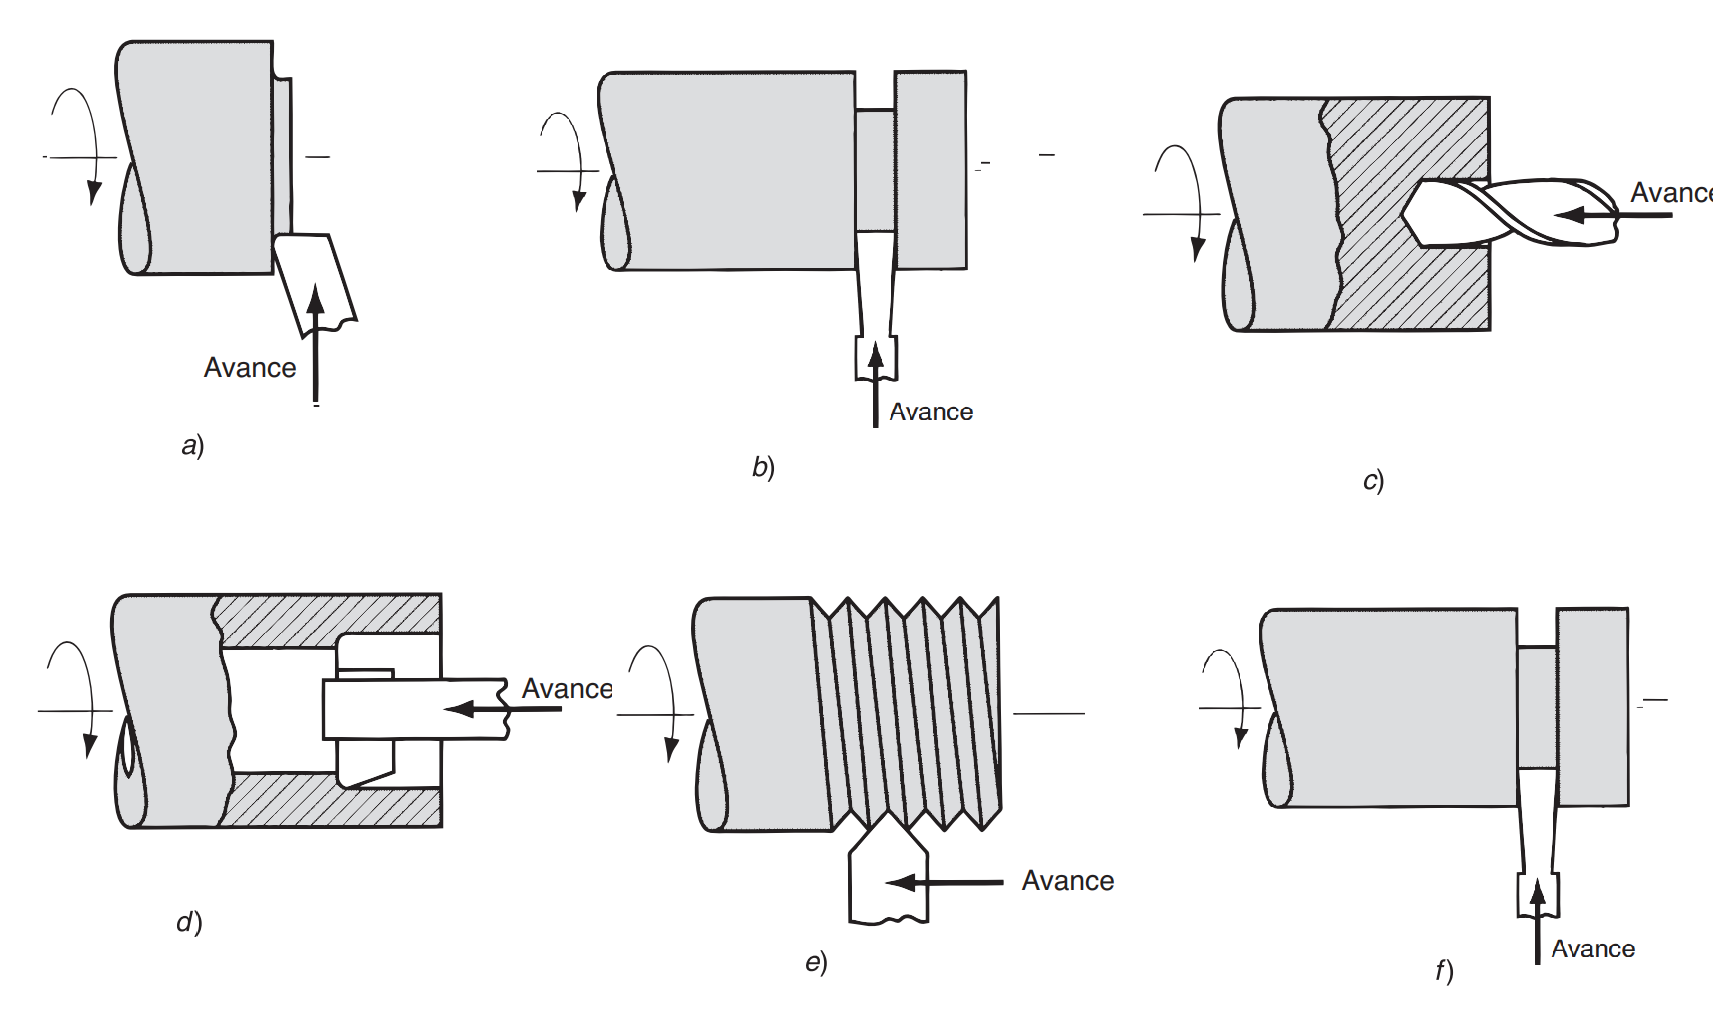
\includegraphics[scale=0.7]{Imagenes/cap3/mecanizado.png} }
\caption{MB7066 XL-MaxSonar-WRL1}{\textbf{Fuente:}, \cite{maxbotix-inc-2019}}.
\label{fig:torneado}
\end{figure}

\begin{figure}[H]
\centering
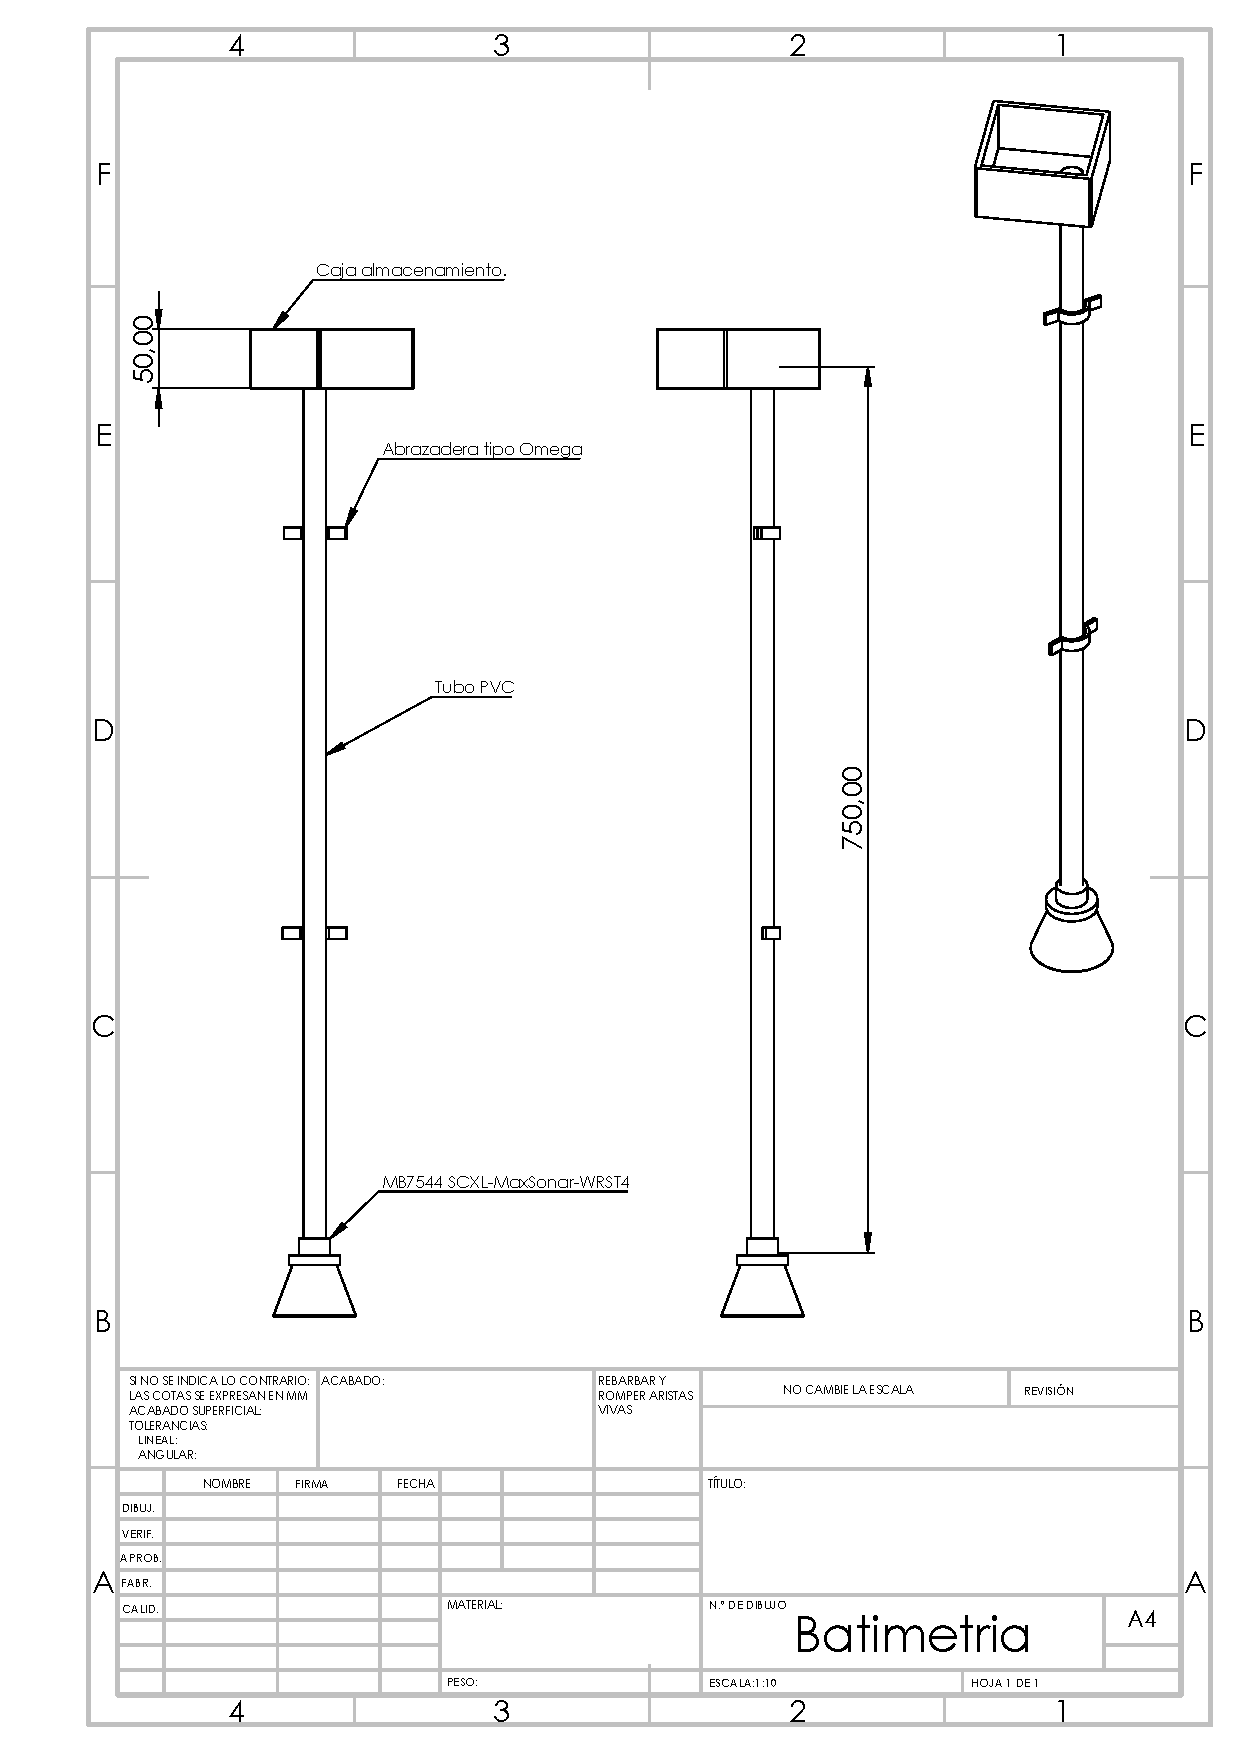
\includegraphics[width=0.9\linewidth]{Imagenes/cap3/Batimetria.pdf}
\caption{Dise\~no final de medidor de profundidad. }{\textbf{Fuente:} elaboración propia}
\label{fig:batimetro}
\end{figure}
\section{Gr\'ua}
Este elemento consiste en un dispositivo pensado para lograr la capacidad de sensado a multinivel, mediante el control de un motor el\'ectrico para el ascenso y descenso de un cabo donde en uno de sus extremos estar\'a instalada la sonda para el  muestreo a diferentes profundidades, el dispositivo se instalar\'a de forma fija en la parte posterior del Cormoran III tal como se puede visualizar en la figura \ref{fig:cormoranMotor}.
Para el desarrollo se consider\'o la adaptaci\'on de un motor el\'ectrico comercial, siendo la mejor opci\'on los del tipo cabrestantes, utilizados por lo general en pequen\~nas embarcaciones para el manejo del ancla. Ppara el correcto dimensionamiento se tuvo en cuenta la tracci\'on m\'inima necesaria para poder extraer la sonda el agua, adem\'as que el voltaje de operaci\'on se encuentre lo m\'as cercano a los 12 voltios, que es el voltaje de almentaci\'on de Cormoran III.
El cabrestante seleccionado fue el TRAC Pontoon35 (figura \ref{fig:cormoranMotor}) que est\'a configurado con un motor DC con reductora, el sistema de originalmente se operaba mediante botones tipo PushButton ubicados en la carcasa con las funciones de ascenso y descenso, mediante la inversi\'on de polarizaci\'on con reles, su voltaje de operaci\'on es de 12 voltios DC y soporta una carga m\'axima de 35Lb.
Para el control, comunicaci\'on y sincronización fue necesario agregar una nueva sistema de accionamiento, distinto con el que viene de fábrica, de tal forma que se pueda operar la gr\'ua de forma autom\'atica y se pueda comunicar con los dem\'as perif\'ericos. 
Para ello se consideró el uso de dos placas extras, uno para el control de potencia del motor, de esta forma controlar las velocidades de subida y bajada, el driver de motor dc utilizado es de la marca Cytron, con una capacidad m\'axima de 30 amper a ser controlado por un microcontrolador, consistente al nodeMCU donde estar\'a cargada el programa principal y estableciera la comunicaron de transmici\'on y recepción de informaci\'on mediante su antena wifi que tiene incorporado. 
Con este nuevo sistema de accionamiento se logrará conectar el módulo gr\'ua en una red para enlazar con los dem\'as perif\'ericos de una forma sencilla.
En el siguiente figura, se puede observar el flujo del software a ser cargado en el nodeMCU,
% e= densidad * volumen * gravedad 
% densidad del teclon 2.2 g/cm³

%%%% INSERAR IMAGEN Y CUADRO DEL PRODUCTO 

\begin{figure}[H]
\centering
\fbox{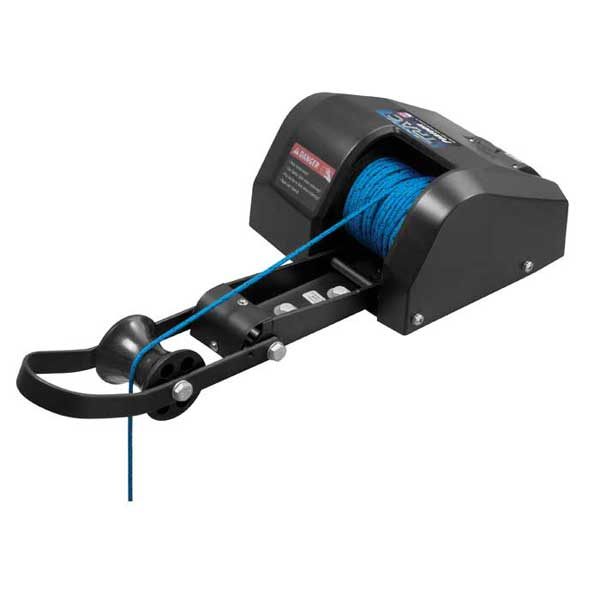
\includegraphics[scale=0.3]{Imagenes/cap3/grua.jpg}}
\caption{Gr\'ua. }{\textbf{Fuente:} Extra\'ido del fabricante \cite{westmarine_trac_nodate}}
\label{fig:cormoranMotor}
\end{figure}

\begin{table}[H]
\caption{Especificaciones de la gr\'ua }
\label{tab:cabrestante }
\centering
\begin{tabular}{ll}
%\hline  
\toprule
\multicolumn{2}{l}{Especificaciones del cabrestante el\'ectrico Pontoon 35}   \\ [1ex] 
%\hline
\midrule
Amperaje                  & 15  {[}A{]}         \\
                          &                     \\
Voltaje                   & 12 {[}V{]}          \\
                          &                     \\
Diámetro                  & 3/16"              \\
                          &                     \\
Dimensiones [AxHxL] & \begin{tabular}[c]{@{}l@{}}$9\frac{3}{4}$" x $5\frac{3}{4}$" x  $19\frac{1}{2}$" \end{tabular} \\
                          &                     \\
Material                  & Acero - Platica ABS \\
                          &                     \\
Tracci\'on m\'axima           & 100 libras          \\
                          &                     \\
Eslora m\'inima del barco   & 20 pies             \\
                          &                     \\
Eslora m\'axima del barco   & 24 pies             \\
                          &                     \\
Velocidad de recuperaci\'on & 65 pulg/min         \\
                          &                     \\
Velocidad de fondeo       & 70 pulg/min         \\ \bottomrule
%\hline
\end{tabular}
\end{table}

En la tabla \ref{tab:cabrestante }  se pueden observar las especificaciones t\'ecnicas del cabrestante eléctrico, el cual cumple con todos los requisitos necesarios para la implementación del sistema de despliegue. 
%%%%%%%%%%%%%%%%%%%%%%%%%%%%%%%%%%%%%%%%%%%%%%%%%%%%%%%%%%%%%%%%%%%%%
 
%% interfaz 

\section{Dise\~no Interfaz}
En este apartado se abordar\'a los criterios y tecnolog\'ias utilizadas para lograr uno de los objetivos proyectos en el desarrollo de este TFG. Como parte del algoritmo de la sonda es almacenar los data recolectados en una base de datos local y además enviarlos a la estación remota vía mqtt, poder visualizar estos datos en una interfaz simple se considera importante, ya que el usuario podr\'ia ver en tiempo real los datos recolectados por la sonda. Por ese motivo, para este trabajo se plante\'o la incorporación de una interfaz gráfica básica, que luego pueda tener otras funcionalidades.
Los criterios que se tuvo en cuenta al momento del diseño e implementación de una interfaz fueron:
\begin{itemize}
    \item multiplataforma: el software multiplataforma o multiplataforma es un tipo de aplicación/programa/software que se ejecuta en múltiples sistemas operativos o dispositivos, comúnmente denominados plataformas. Plataforma se refiere a un sistema operativo como Windows, Mac OS, Android o iOS. Cuando una aplicación funciona en múltiples plataformas, los usuarios pueden usar ese software en muchos dispositivos y computadoras diferentes, \cite{roca_que_2020}. Con esto, la curva de aprendizaje de uso podría reducirse por utilizar en un dispositivo en el cual ya te encuentras familiarizado. 
    \item open source: los proyectos, productos o iniciativas de código abierto adoptan y celebran los principios de intercambio abierto, participación colaborativa, creación rápida de prototipos, transparencia, meritocracia y desarrollo orientado a la comunidad, \cite{opensourcecom_camino_nodate}. Sus autores ponen su código fuente a disposición de otras personas que deseen ver ese código, copiarlo, aprender de él, modificarlo o compartirlo. Adem\'as de los costos ahorrados en conceptos de licencias,   
    \item escalable: para este trabajo, se promueve una interfaz gr\'afica sencilla con el cual el principal objetivo es que el usuario pueda previsualizar, las lecturas de los par\'ametros recolectados en tiempo real. En un futuro se espera que la interfaz pueda realizar m\'as funciones, los cuales no se abordaran en este trabajo.
    \item liviano: se espera que la interfaz gr\'afica pueda ser compatible y ejecutado en dispositivos como ser un raspberry pi, donde los recursos son limitados.
\end{itemize}
Tendiendo en cuenta los criterios expuestos, se opt\'o por el uso de la tecnolog\'ia Node-RED que es una herramienta web de programación basada en flujo, desarrollada originalmente por el equipo de Servicios de Tecnología Emergente de IBM y ahora parte de la Fundación OpenJS.
La programaci\'on basada en flujo, fue inventada por J. Paul Morrison en la década de 1970, la programación basada en flujo es una forma de describir el comportamiento de una aplicación como una red de cajas negras o “nodos”, como se denominan en Node-RED. Cada nodo tiene un propósito bien definido; se le dan algunos datos, hace algo con esos datos y luego los pasa. La red es responsable del flujo de datos entre los nodos, \cite{noauthor_about_nodate}.
Node Red, es un de código abierto desde septiembre de 2013. El entorno de ejecución ligero se basa en Node.js y aprovecha al máximo su modelo sin bloqueo basado en eventos. Esto lo hace ideal para ejecutarse en el borde de la red en hardware de bajo costo como Raspberry Pi, así como en la nube. Con más de 225 000 módulos en el repositorio de paquetes de Node, es fácil ampliar el rango de nodos de paleta para agregar nuevas capacidades.

\begin{figure}[H]
    \centering
    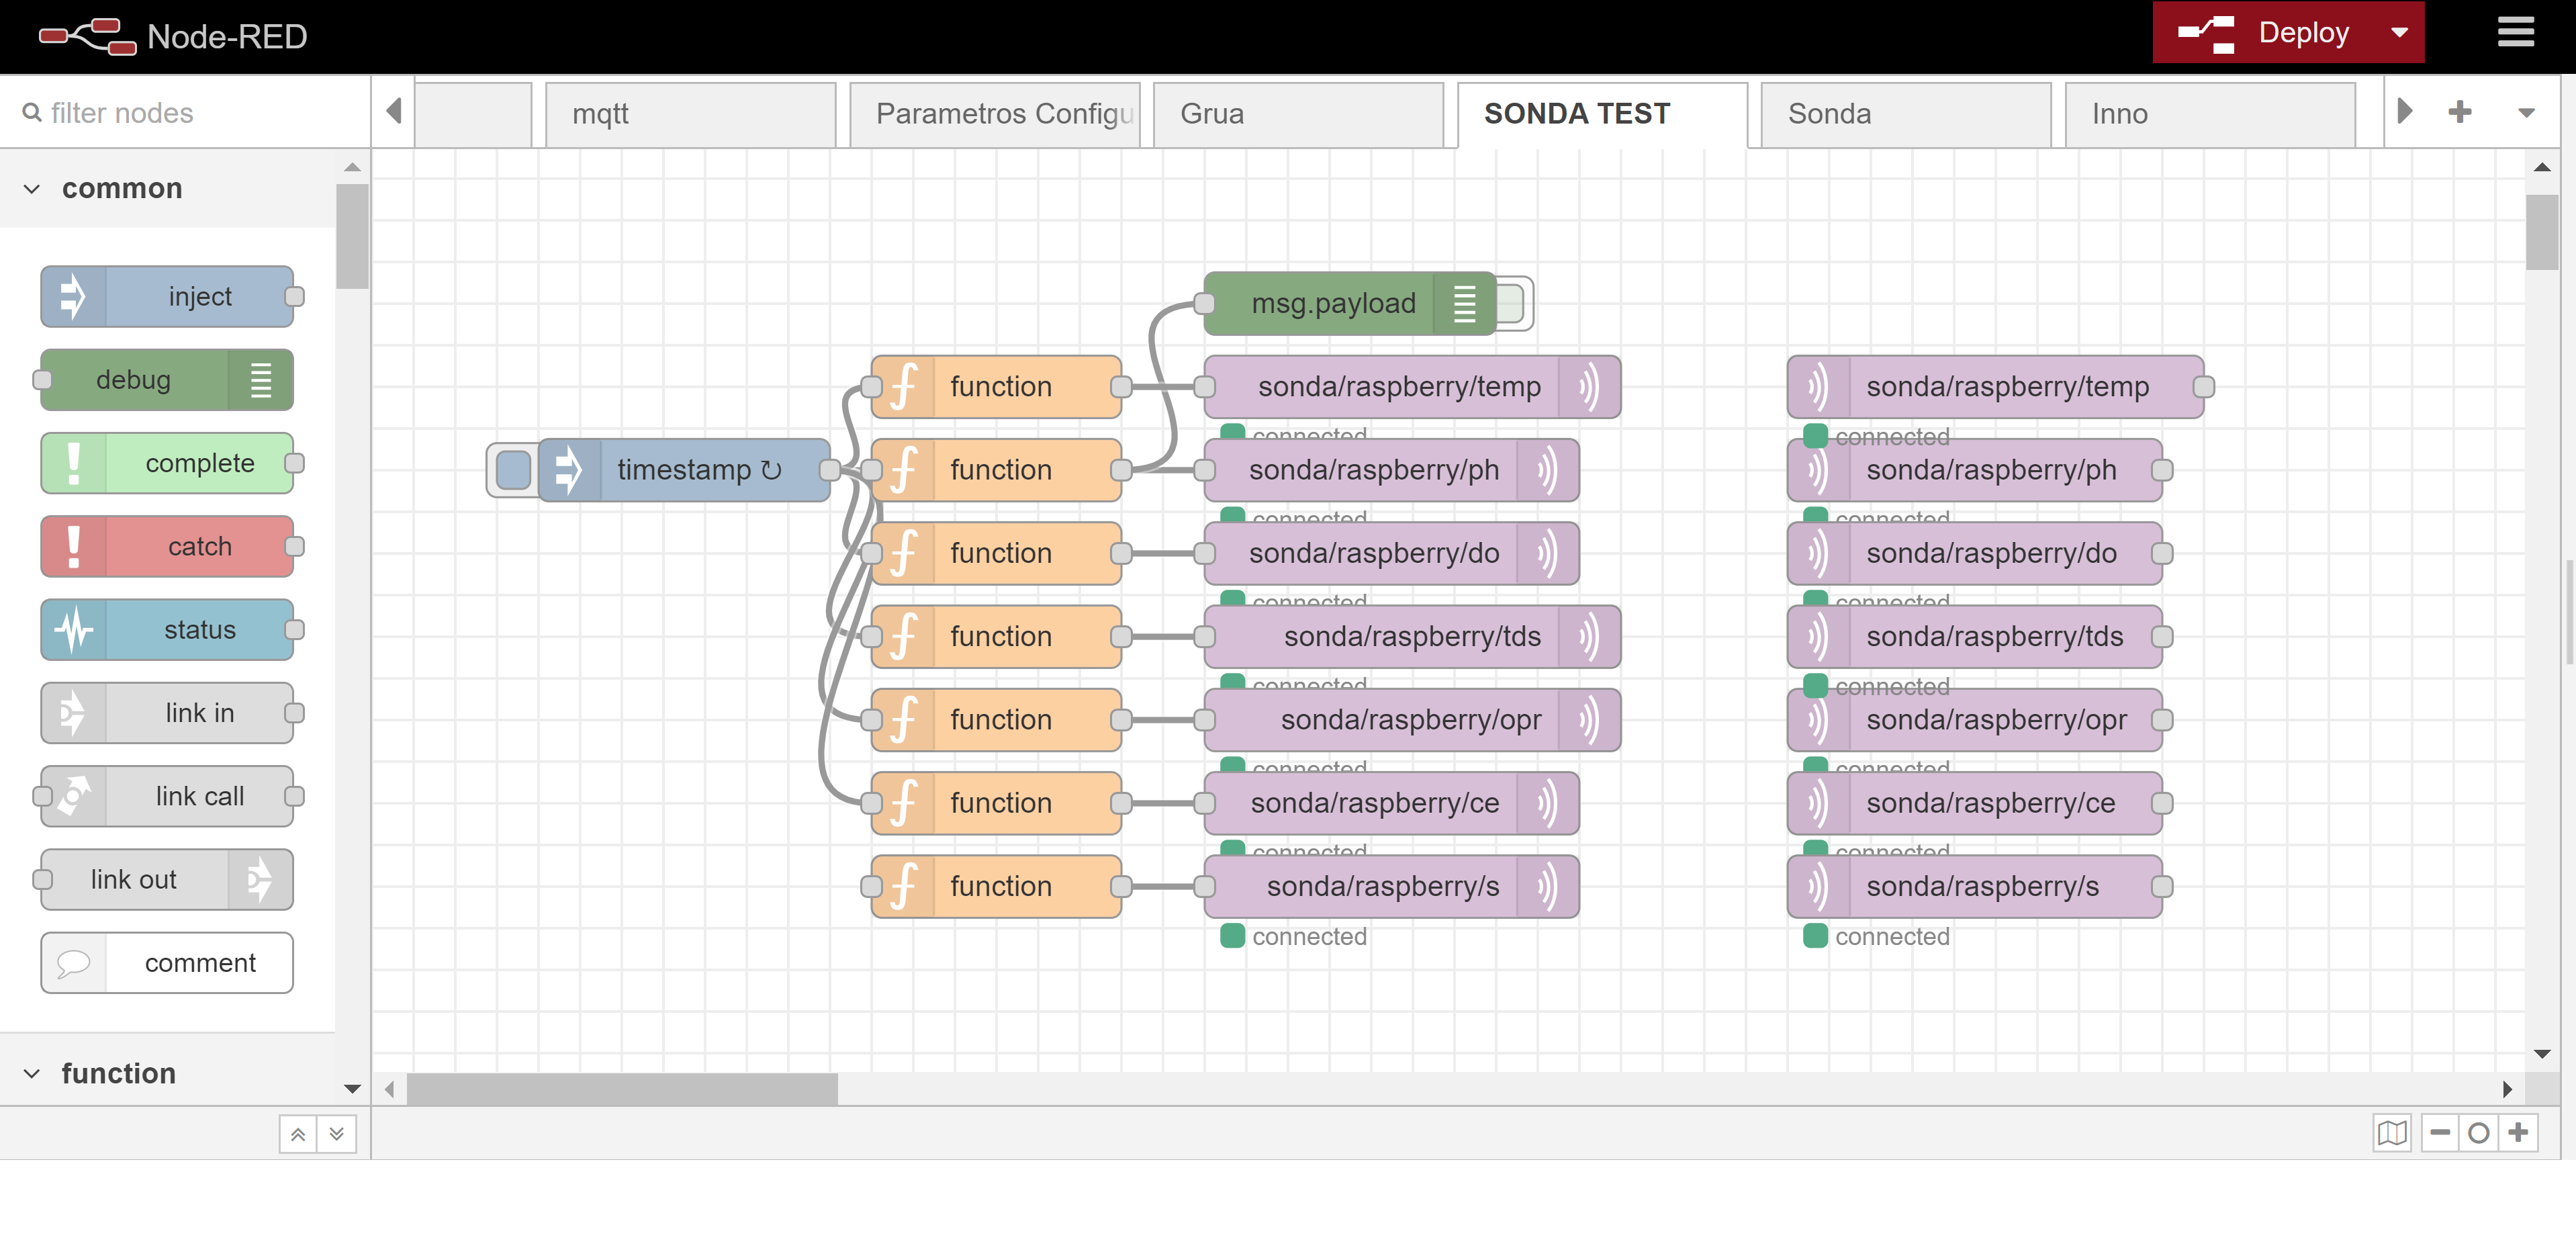
\includegraphics[width=0.75\linewidth]{Imagenes/cap3/flujoNode_red.png}
    \caption {Programaci\'on basada en flujo sensores de sonda. }{\textbf{Fuente:}
    Elaboraci\'on Propia. }
    \label{fig:M1CE}
\end{figure}

Como fue dise\~nada espec\'ificamente para visualizar y manipular asignaciones entre t\'opicos de MQTT, algunos nodos de aplicaciones de servicios de red b\'asicos, como HTTP y WebScoket, Node-RED tambi\'en brinda soporte de acceso al protocolo MQTT. 
Lo que lo hace ideal y compatible con el protocolo de comunicaci\'on que utiliza la sonda, Node-RED proporciona un nodo\'on se usa para la entrada de datos, mientras que el nodo de publicaci\'on se puede usar para la salida de datos.